\documentclass[12pt]{article}
\usepackage[a4paper]{geometry}
\usepackage[dvipsnames]{xcolor}
\usepackage{lipsum}
\usepackage{framed}
\usepackage{graphicx}
\usepackage[basque]{babel}
\usepackage{setspace}
\usepackage{verbatim}
\usepackage{hyphenat}
\usepackage{indentfirst}
\usepackage{booktabs}  
\usepackage{fancyvrb}
\usepackage{tikz}
\usetikzlibrary{trees}
\usepackage[table]{xcolor}
\usepackage{subcaption}
\usepackage[dvipsnames]{xcolor}
\usepackage{amsmath}
\usepackage{amssymb}
\usepackage{extpfeil}
\usepackage{siunitx}
\usepackage{multicol}
\sisetup{output-decimal-marker = {,}}
\usepackage{wrapfig}
\setlength{\parindent}{20pt}
\usepackage[style=ieee, sorting=none, biblabel=brackets]{biblatex}
\ExecuteBibliographyOptions{date=year}
\addbibresource{tfgelectronica.bib}
\AtEveryBibitem{
  \clearfield{doi}
  \clearfield{issn}
  \clearfield{isbn}
  \clearfield{note}
  \clearfield{urldate}
}
\usepackage{enumitem}
\usepackage{caption}
\setlength{\aboverulesep}{0pt}
\setlength{\belowrulesep}{0pt}
\usepackage{fontspec}
%%%%%%%%%%%% LETRAREN ITURRIA ALDATZEKO (EHUSerif) %%%%%%%%%%%%
\setmainfont{EHUSerif-Light.otf}[ % Nombre completo del archivo Regular
  Path = ./EHU Serif/,                        % Cambia esto si las fuentes están en una subcarpeta
  BoldFont = EHUSerif-Regular,     % Nombre completo del archivo Bold
  ItalicFont = EHUSerif-Italic, % Nombre completo del archivo Italic
  BoldItalicFont = EHUSerif-BoldItalic, % Nombre completo del archivo BoldItalic
]
\newfontface\lightfont{EHUSerif-Light.otf}[Path=./EHU Serif/]
\newfontface\blackfont{EHUSerif-Black.otf}[Path=./EHU Serif/]
\numberwithin{figure}{section}
\numberwithin{equation}{section}

\addto\captionsbasque{%
  \renewcommand{\figurename}{irudia}
}

\makeatletter
\renewcommand{\fnum@figure}{\textbf{\thefigure\ \figurename}}
\makeatother

\addto\captionsbasque{%
  \renewcommand{\tablename}{taula}
}
\makeatletter
\renewcommand{\fnum@table}{\textbf{\thetable.\ \tablename}}
\makeatother

\newcommand\blankpage{%
    \null
    \thispagestyle{empty}%
    \addtocounter{page}{-1}%
    \newpage}

\geometry{top=2.5cm, bottom=2.5cm, left=2.5cm, right=2.5cm}
\begin{document}
\setstretch{1.0}
\definecolor{light-gray}{gray}{0.87}  

\begin{titlepage}
\hspace*{-3.5cm}
    \begin{minipage}{\textwidth}
        \vspace{-2.5cm}
        \begin{center}
    

            
\includegraphics[width=\paperwidth]{LogoEHU.PNG}
        \end{center}
    \end{minipage}

\vspace{1cm}

\hspace{-3.5cm}
\noindent\fcolorbox {light-gray}{white}{

    \parbox{\paperwidth}{
     \begin{center}
     \large Gradu amaierako lana\\
     \large Ingeniaritza Elektronikoko Gradua
     \end{center}
    }
    }


\vspace{0.8cm}

\noindent\hspace*{-2.5cm}%
\colorbox{light-gray}{\begin{minipage}{\paperwidth}%

    \vspace{1cm}

    \color{RoyalBlue}
    \centering\Large\textbf{ECR ioi-iturrien plasma-trantsizioak eta sentsore akatsak modu ez-intrusiboan automatikoki detektatzeko sistema orokorra}
    \\


    \vspace{8cm}\mbox{}
  \end{minipage}
}
\vspace{0.8cm}

\begin{flushright}
 Egilea:
\\
Urko Lopez Sacristan
\\
Zuzendariak:
\\
Iñigo Arredondo López de Guereñu
\\
Raquel Justo Blanco                 
\\
\end{flushright}

\vspace{1cm}

\hspace{-3.5cm}
\noindent\fcolorbox {light-gray}{white}{
    \begin{minipage}[]{1000pt}

        \parbox{\paperwidth}{
            \begin{center}
    
                 Leioa, 2025eko ekainaren 20a

            \end{center}
        }
    \end{minipage}
}
\end{titlepage}


%%%%%%%%%%%%%%%%%%%%%%%%%%%%%%%
%Hemendik aurrera hasi lana idazten%
%%%%%%%%%%%%%%%%%%%%%%%%%%%
\blankpage

\tableofcontents
\thispagestyle{empty}
\setcounter{page}{0}
\newpage

\section{Sarrera}
1927an, Ernest Rutherfordek laborategietan partikulak energia altuetara azeleratzeko beharra azpimarratu zuen, garaian desintegrazio erradioaktibo naturaletatik sortutako partikulak baino ez zirelako erabilgarriak \cite{rutherford_address_1997}. Horri erantzunez, eta soilik bost urte geroago, Cockroft eta Waltonek tentsio altuak lortzeko zirkuitu biderkatzaile bat diseinatu eta hidrogenotik sortutako protoiak 200 kV-etara azeleratzea lortu zuten \cite{cockcroft_experiments_1997}. \\

Ordutik, partikula azeleragailuen teknologia etengabe garatu da, izpien energiak keV-etatik TeV-etara igaroz, eta funtsezko tresnak bihurtu dira energia altuko fisikaren ikerkuntzan. Horren adibide esanguratsuena da 2012an LHC azeleragailuan Higgs bosoiaren existentziaren lehen froga esperimentala \cite{aad_observation_2012}. \\

Hala ere, horien erabilera ez dago oinarrizko fisikaren ikerkuntzara mugatuta. Areago, munduan existitzen diren 50000 partikula-azeleragailuetatik erdia industria aplikazioetan erabiltzen dira, ioi-ezarpenerako batez ere, eta gainontzeko handia berriz medikuntza aplikazioetan, radioterapian bereziki \cite{sheehy_applications_2024}. Aplikazio aniztasun handi honek etengabeko garapena eskatzen du, bi helburu nagusirekin: alde batetik, errendimendua eta kalitatea hobetzea; eta bestetik, eskuragarritasuna hobetzea, azeleragailu txikiago eta merkeagoak eraikiz.

\subsection{Linac-7 proiektua}
\label{sec:sarrera}
Premia horiek asetzeko, 2018an Euskal Herriko Unibertsitateko IZPILab Laborategiak Linac-7 proiektua azaleratu zuen, bertako hainbat industria-enpresen lankidetzarekin \cite{feuchtwanger_new_2022}. Proiektuaren helburua, izenak berak islatzen duen moduan, energia eta intentsitate baxuko protoi azeleragailu lineal bat diseinatzea eta eraikitzea da, ahalik eta trinkoena eta merkeena izanik. Horrez gain, Euskal Herrian partikula azeleragailuetan aditua den ikerketa-talde bat eratzea du helburu ere.\\

Linac-7-ren aplikazio nagusiena PET (\textit{Positron Emission Tomography}) diagnostikoarentzat beharrezkoak diren erradiofarmakoak produzitzea da \cite{victor_etxebarria_manufacturing_2022}. Gaur egun, aktibitate handiko eta erdibizitza luzeko erradioisotopo kaltegarriak erabiltzea ohikoa da, sortze-zentroetatik ospitaleetara garraiatu behar baitira. Ondorioz, proiektuaren kostu eta tamainaren funtsezko abantaila pazienteentzako berehalako dosiak lokalki sortzea da. Protoientzat aukeratutako 7 MeV-eko energiari esker, erdibizitza laburreko positroi-igorle ugari sor daitezke, hala nola $^{18}F$, $^{15}O$, $^{13}N$ eta $^{11}C$.\\

Esperotako energia lortzeko, azeleragailua sei etapaz osatzen da (1.1 Irudia):
\begin{enumerate}[itemsep=0em, topsep=0.8em]
    \item \textbf{\textit{Electron Cyclotron Resonance}} (ECR) ioi-iturria.
    \item \textbf{\textit{Low Energy Beam Transport}} (LEBT).
    \item \textbf{\textit{Radio Frequency Quadrupole}} (RFQ).
    \item \textbf{\textit{Medium Energy Beam Transport}} (MEBT).
    \item \textbf{\textit{Drift Tube Linac}} (DTL).
    \item \textbf{\textit{Beam Stop}}.
\end{enumerate}

\begin{figure}[h]
    \centering
    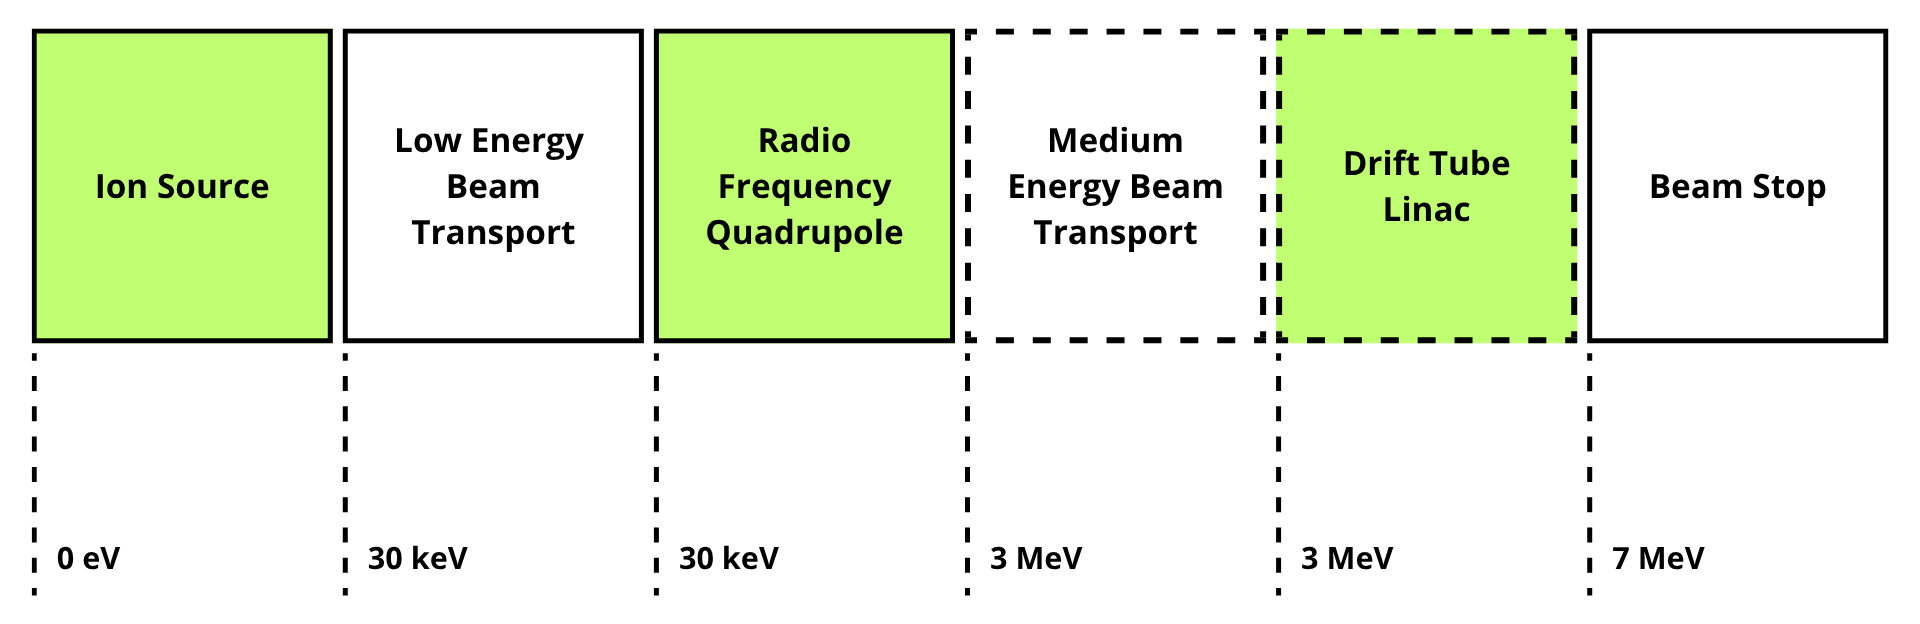
\includegraphics[width=\linewidth]{1 - Sarrera/etapas linac7.png}
    \caption{Linac-7 azeleragailuaren etapen eskema sinplea. Ertz eteneko etapak ez daude eraikita. Atzekaldea kolorezkoa dutenak azelerazio etapak dira.}
    \label{fig:linac7etapak}
\end{figure}
Lehenik eta behin, mikrouhinekin sortutako hidrogeno plasma batetik ioiak erauzten dira, 30 kV-eko elektrodo bat erabiliz. Ondoren, LEBT sistemak izpia solenoideen bidez egokitzen du RFQ-ra sartzeko egokia izan dadin, bertan 3 MeV-etaraino azeleratuko baita. MEBT-ak berriz ere izpia doitzen du hurrengo etapa azeleratzailera sartu baino lehen, bukaeran 7 MeV-eko energia lortuz, eta azkenik, izpia segurtasunez gelditzen da.\\

Lehenengo hiru etapak jada eraikita daude eta proba ugari aurrera eraman dira, baina MEBTa eta DTLa oraindik diseinu fasean daude. Testu honetan lehenengo bi etapetan soilik sakonduko da.

\subsection{ECR eta Plasma}
\label{sec:ecrplasma}

Edozein azeleragailuren lehen osagaia ioi-iturria da. Kasu honetan, PIT30 deituriko ioi-iturria erabiltzen da (\textit{Protoi Iturri Trinkoa 30 keV}) \cite{elorza_romera_pit30_2021} elektroien ziklotroi-erresonantzia (ECR) erabiliz plasma ionizatzeko eta bertatik ioiak erauzteko (\ref{fig:pit30iturria}. irudia). \\

ECR ioi-iturrietan eremu magnetiko konstante bat ($\Vec{B}$) sortzen da plasma\hyp{}ganberan, eta horren eraginpean, elektroi askeek Lorentzen indarra jasaten dute, eremu horri perpendikularra den ibilbide zirkular bat deskribatuz. Biraketa maiztasunari ziklotroi-maiztasuna ($f_{ce}$) deritzo,\\

\begin{equation}
    f_{ce} = \frac{eB}{2\pi m_{e}}
\label{eq:ziklotroi}
\end{equation}
\\
non $e$ eta $m_e$ elektroiaren karga eta masa diren, hurrenez hurren. Orduan, ganberari eremu magnetikoaz gain kitzikapen elektromagnetiko bat transmitituz gero, kitzikapenaren maiztasuna ($f_{EM}$) ziklotroi-maiztasunarekin bat badator, ECR erresonantzia agertzen da: elektroiek energia handia irabazten dute. Beraz, plasma-ganberan gas bat injektatuz gero, elektroiek atomo neutroak ionizatzen dituzte, karga positiboak eta negatiboak banatuz, eta plasma sortuz.

\newpage
PIT30-ren kasuan, erresonantzia 3 GHz-ko maiztasunean gertatzeko diseinatuta dago, ganberan $TE_{111}$ modoa kitzikatuz. \eqref{eq:ziklotroi} ekuazioaren arabera, elektroiek maiztasun horretan biratzeko beharrezko eremu magnetikoaren intentsitatea $B=110mT$ ingurukoa izan behar da.

\begin{figure}[h]
    \centering
    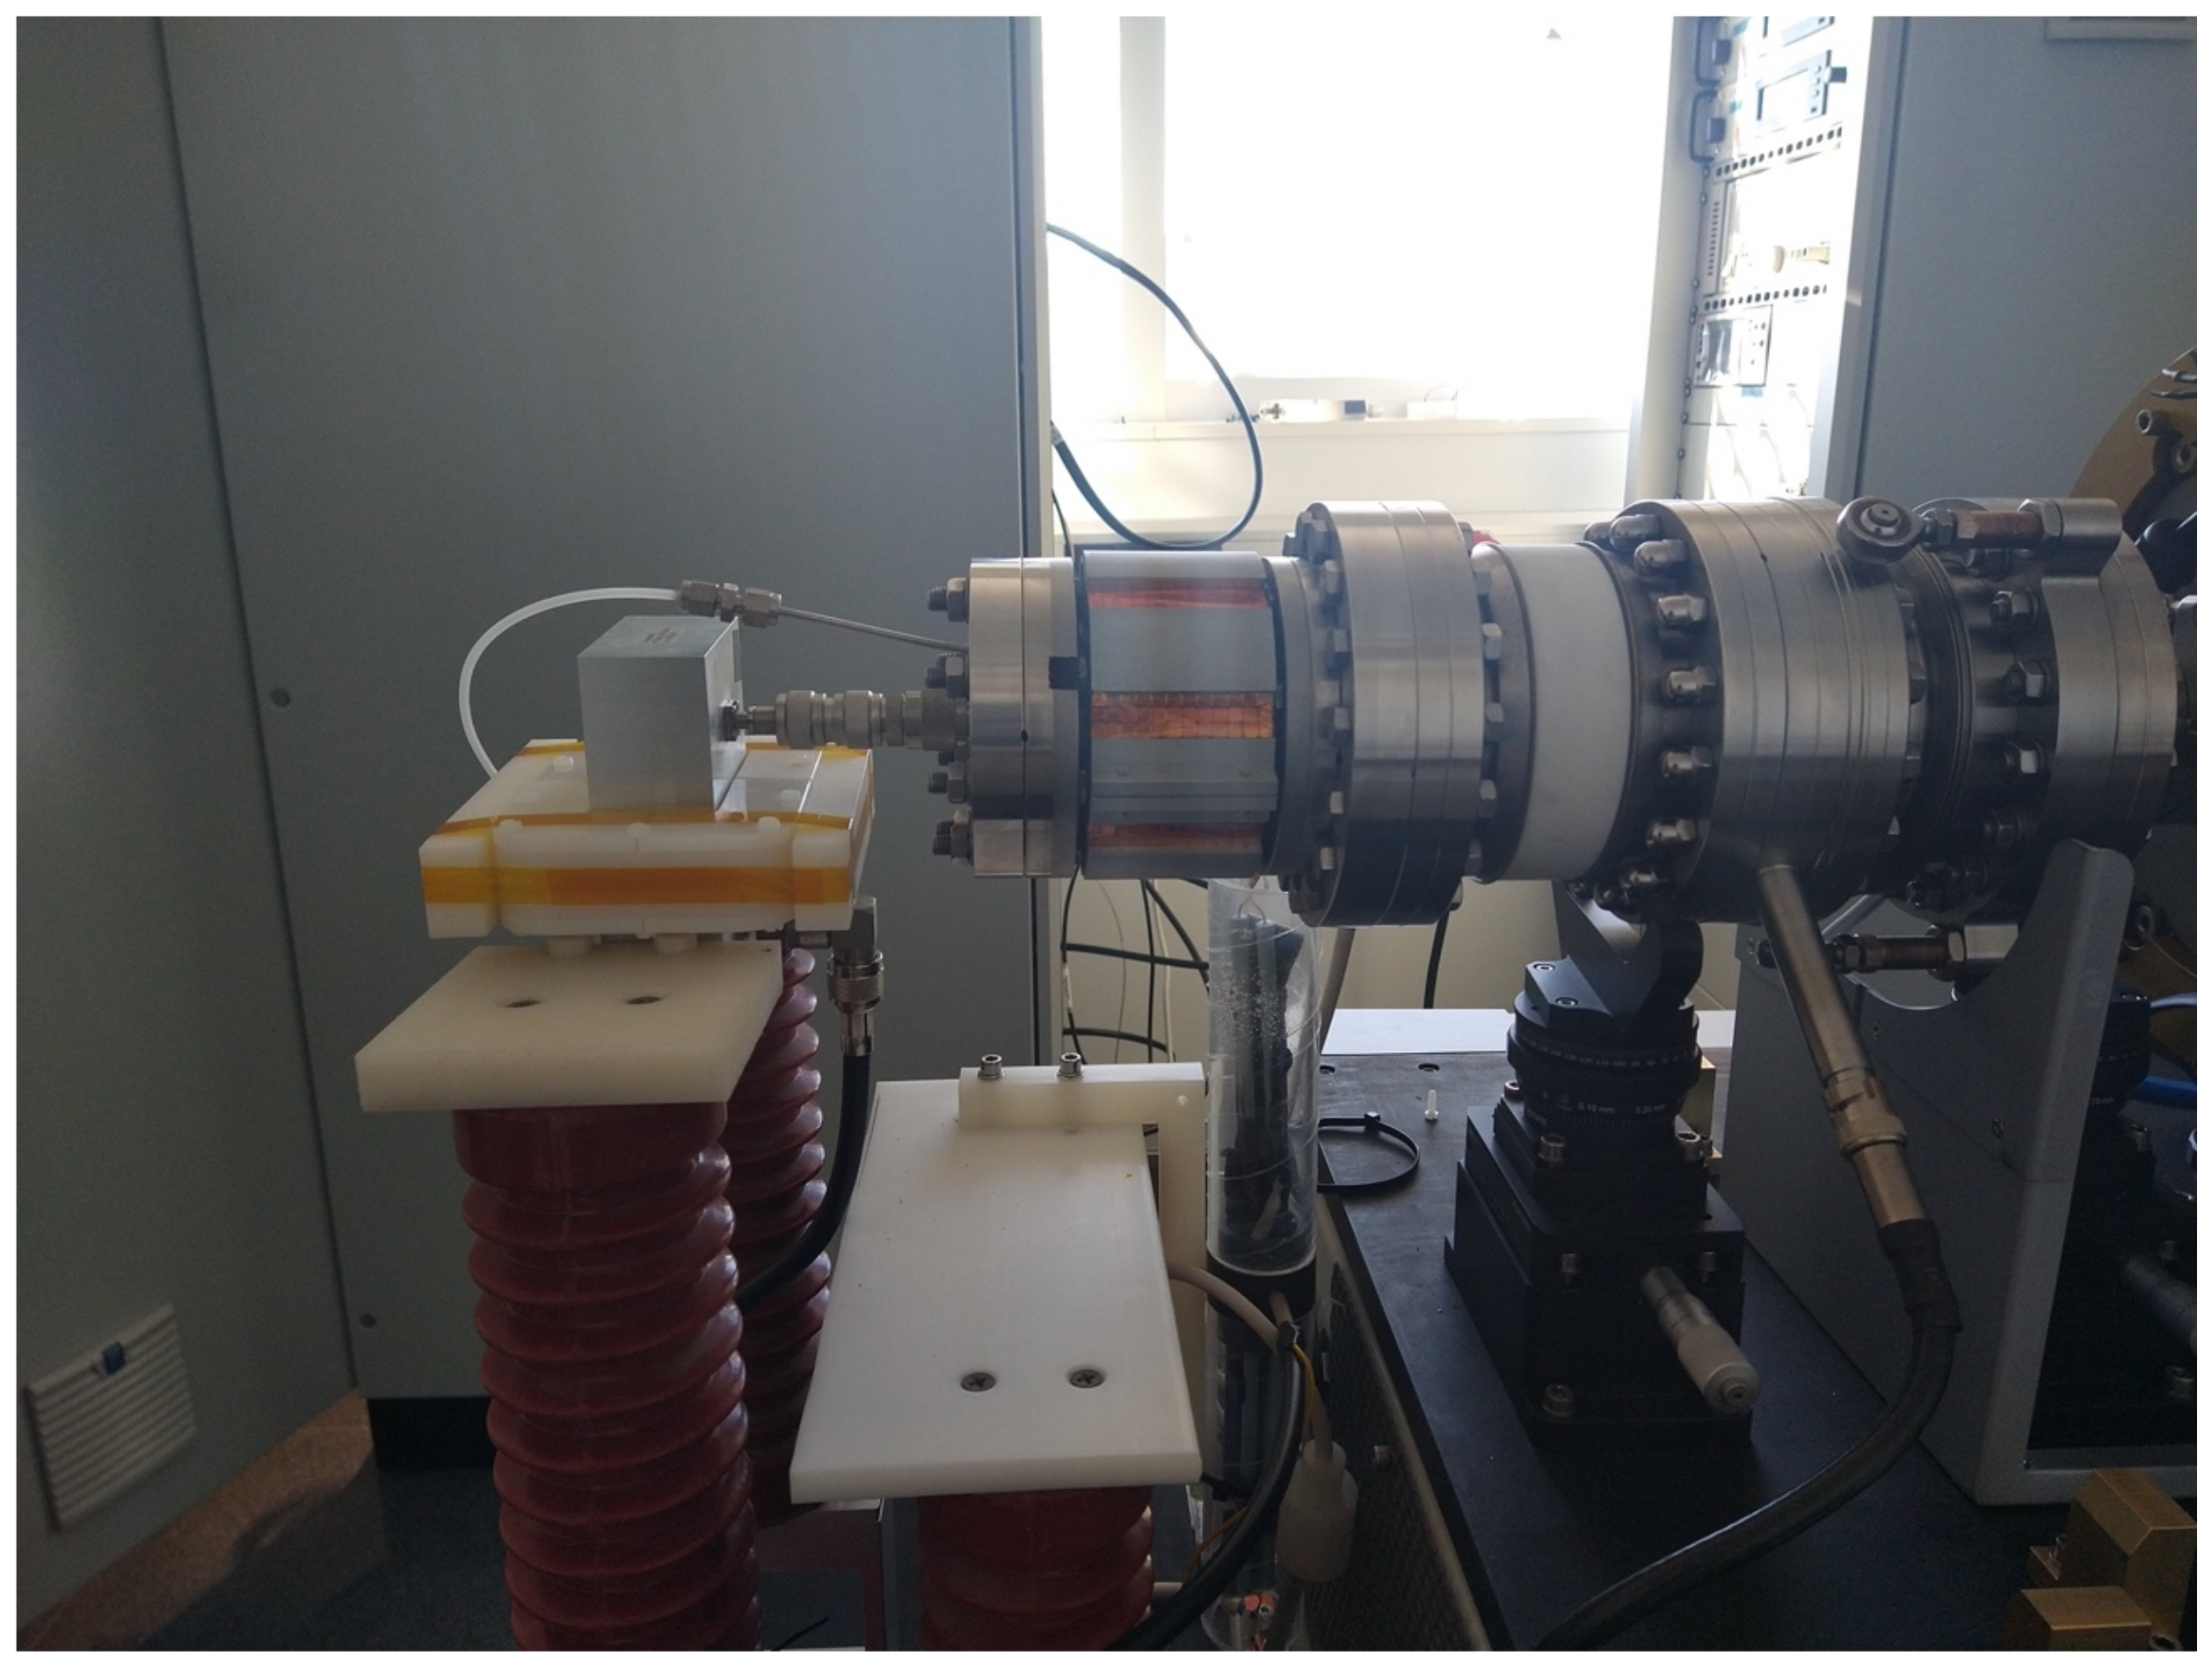
\includegraphics[width=0.5\linewidth]{1 - Sarrera/pit30argazkia.png}
    \caption{PIT30 ioi-iturriaren argazkia \cite{feuchtwanger_new_2022}.}
    \label{fig:pit30iturria}
\end{figure}

Iturri honetan plasma sortzeko erabiltzen den gasa hidrogenoa da, $H_2$, eta plasmaren erreakzioetan protoiak ($H^+$) sortzen dira. Beste hidrogeno espezie batzuk ere sortzen dira ($H_2^+$, $H_3^+$, $H$), eta ikusi da ganberara transmititutako RF potentziaren arabera eta gas-fluxuaren arabera espezie batzuen sorkuntza beste espezieen aurrean gailentzen dela (\ref{fig:mapa}. irudia) \cite{elorza_romera_modelo_2022}.

\begin{figure}[h]
    \centering
    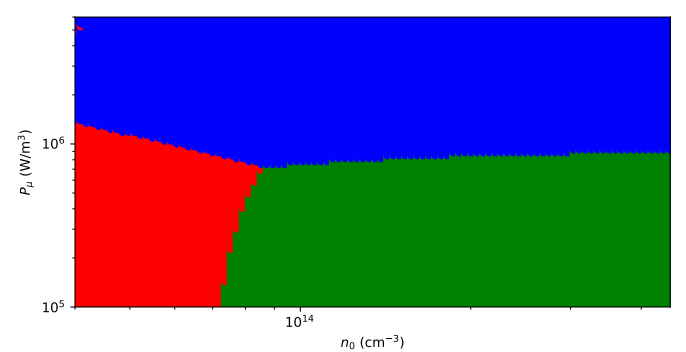
\includegraphics[width=0.8\linewidth]{1 - Sarrera/predominant_map.PNG}
    \caption{Espezie bakoitza (\colorbox{cyan}{$\mathbf{H_{ }^+}$}, \colorbox{red}{$\mathbf{H_2^+}$}, \colorbox{green}{$\mathbf{H_3^+}$}) gailentzen den zonaldeen mapa, potentzia-dentsitatearen eta gas-dentsitatearen arabera.}
    \label{fig:mapa}
\end{figure}
Hori dela eta, plasma-ganberaren egoera monitorizatzea ezinbestekoa da: alde batetik, plasmaren sorkuntzan eta manipulazioan parte hartzen duten dispositibo guztien funtzionamendu egokia ziurtatzeko; eta bestetik, horren egoeraren ahalik eta diagnostikorik onena egiteko.

\subsection{Diagnostiko ez-intrusibo eta automatikoa}
\label{sec:ez-intrusibo}
ECR plasmaren diagnostiko fidagarria egiteko bi modu existitzen dira \cite{tarvainen_plasma_2019}: intrusiboa, zunden bitartez zuzenean neurtuz, eta ez-intrusiboa, plasma-ganberako uhin-elektromagnetikoen analisiaren bidez. Dena dela, zundak barneratzean, plasma sortzeko beharreko eremu magnetikoak aldatzen dira, plasmaren egoera aldatuz ere. Gainera, kasu honetan ganbera trinkoa aukeratu denez, zundek sartutako aldaketak handiegiak dira, eta diagnostiko mota hau ez da erabilgarria \cite{vivas_merino_sistema_2023}.\\

Ondorioz, Linac-7 azeleragailuaren diagnostiko nagusia metodo ez-intrusiboen bidez burutzen da, ioi-iturrira igorritako RF seinalea eta gas-fluxua aztertuz. RF seinalerako, bi detektore berdin existitzen dira (\textit{Pasternack PE8012}\cite{noauthor_schottky_2025}), transmititutako eta islatutako potentziak neurtzeko, eta \textit{NI PXI} \cite{noauthor_sistemas_2025} batera konektatuz datu guztiak kudeatzen dira eta beste magnitude batzuk eratorri ere. Gas-fluxurako, ordea, gas-kontroladore bat (\textit{Omega FMA 2615A}\cite{noauthor_mass_2025}) erabiltzen da, eta RF sorgailuarekin \textit{NI CompactRIO} \cite{noauthor_sistemas_2025-1} batera konektatzen dira. Informazioa bi puntu horietatik jaso eta sare-lokalera konektatutako edozein ordenagailutik eskuratu daiteke (\ref{fig:datu_eskema}. irudia).

\begin{figure}[h]
    \centering
    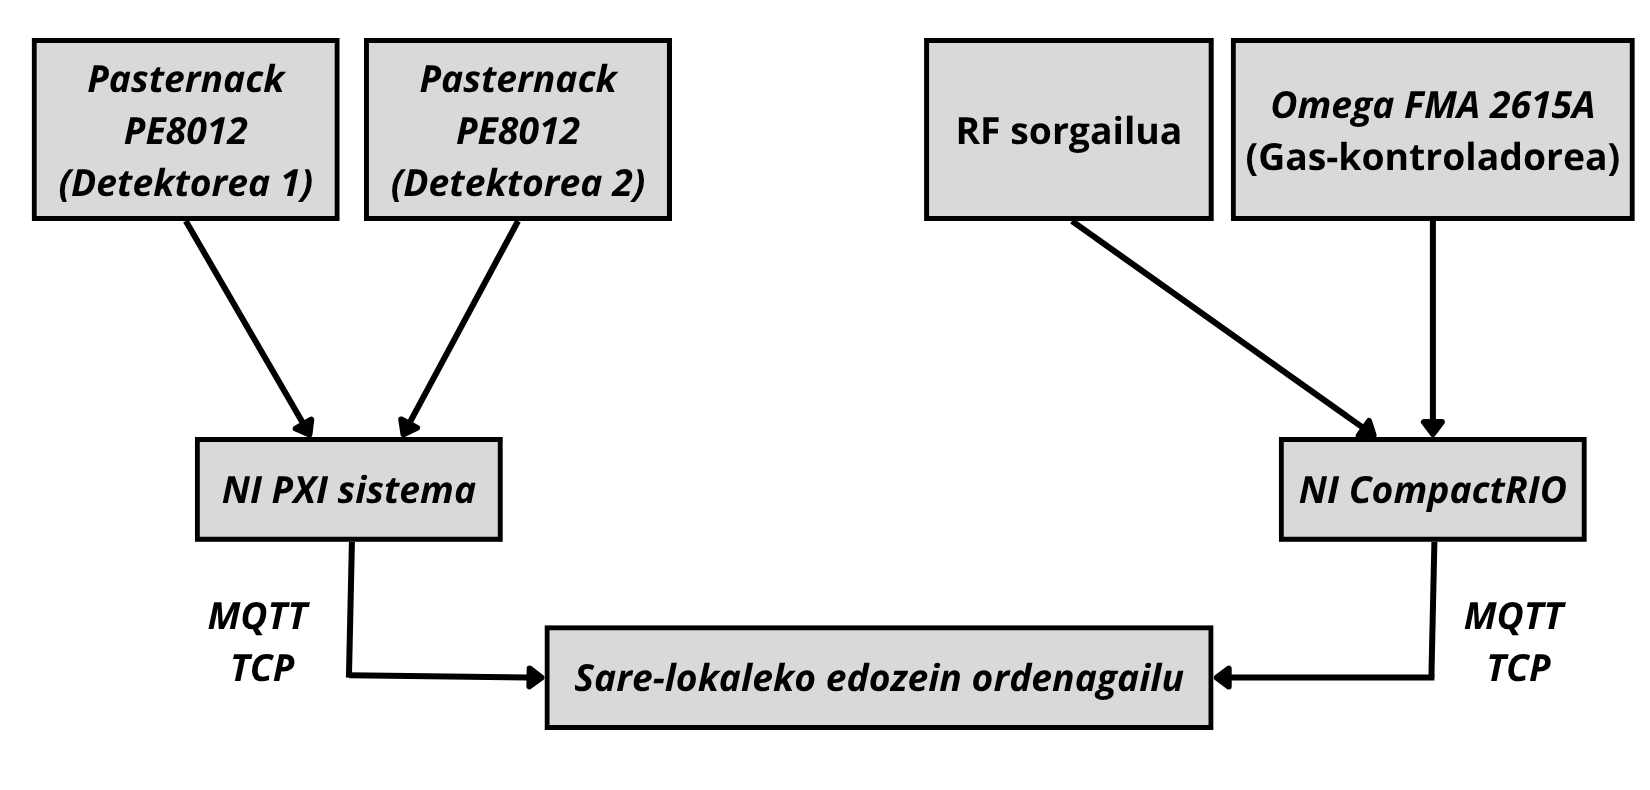
\includegraphics[width=\linewidth]{1 - Sarrera/DATU_ESKEMA.png}
    \caption{Linac-7 proiektuko datu-kudeaketaren eskema.}
    \label{fig:datu_eskema}
\end{figure}

Bestalde, azeleragailuaren garapenean beste diagnostiko bat erabili da ere: argitasuna. CCD kamera baten bitartez (\textit{pco.panda 4.2}\cite{noauthor_pcopanda_2025}), aldagaien balioak egokiak direnean, plasma pizten da, eta LEBT-aren amaieran dagoen irekiera baten ikus daiteke (\ref{fig:plasma_pictures}. irudia). Argitasunaren neurketa oso erabilgarria izan da plasmaren egoera aztertzeko, RF seinalearen potentziaren eta gas-fluxuaren arabera argitasunean jauzi handiak behatzea posiblea izan baita \cite{elorza_romera_pit30_2021}. Testu honetan jauzi horiei \textbf{trantsizio} deituko zaie. \\

\begin{figure}[h]
    \centering
    \begin{subfigure}[b]{0.38\textwidth}
        \centering
        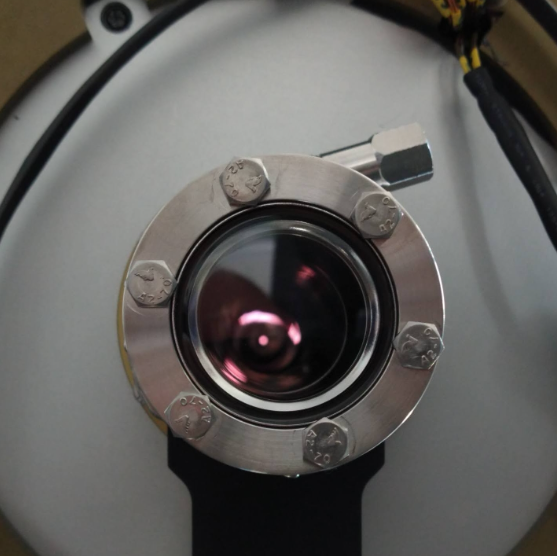
\includegraphics[width=\linewidth]{1 - Sarrera/plasma1.png}
    \end{subfigure}
    \hspace{0.02\textwidth}
    \begin{subfigure}[b]{0.38\textwidth}
        \centering
        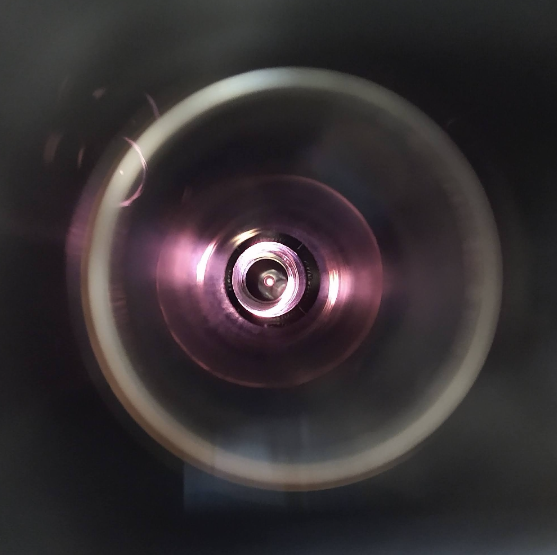
\includegraphics[width=\linewidth]{1 - Sarrera/plasma2.png}
    \end{subfigure}
    \caption{LEBT-aren irteeran behatutako plasmaren argitasuna.}
    \label{fig:plasma_pictures}
\end{figure}

Hala ere, azeleragailuaren hurrengo etapak eraikita daudenean argitasuna neurtzea ezinezkoa izango denez, trantsizioak beste magnitudeekin erlazionatzea lortu da \cite{fernandez_rua_clasificacion_2024}, eta horiek automatikoki detektatzea oso interesgarria izango litzateke, batez ere plasmaren pizketa argitasunik gabe ezagutzeko.\\

Detektoreen eta kontroladoreen egoera kontuan hartzea ere funtsezkoa da; izan ere, ioi-iturriaren luzaroko erabilerak horien higadura sor dezake, magnitudeen neurketak oztopatuz edo zehaztasuna kaltetuz. Hori dela eta, akats edo anomalien detekzioak berebiziko garrantzia du, eta hori automatizatzea oso interesgarria izango litzateke.

\subsection{Helburuak}
Testu honen helburu nagusia ECR motako ioi-iturrien zuzeneko plasma\hyp{}trantsizio eta akatsen detekzio automatikorako zerbitzu bat garatzea da.\\

Sistemaren garapenerako Linac-7 azeleragailuko datuak erabiliko dira eta bertan testatuko da. Beraz, proiektuaren datu-eskuratze sisteman sakonduko da, aldagaiak eta neurtutako magnitudeak ulertuz eta prozesatuz. Gainera, zerbitzua kontrol-sistematik guztiz independentea izango da, azeleragailuaren funtzionamendua oztopatu gabe informazioa prozesatzea ahalbidetuz.\\

Horrez gain, zerbitzua eskalagarria eta ahalik eta orokorrena izatea du helburu ere, hainbat azeleragailu eta inguruneetara egokitzeko, eta ez soilik Linac-7-ra. Horretarako, hainbat teknologia aztertu eta integratuko dira: \textit{MQTT}, datuen komunikaziorako; \textit{InfluxDB}, datu-base moduan; eta \textit{Docker}, sistema modularra eta eramangarria izateko.


\newpage
\section{Ingurunea}
\label{sec:ingurunea}
Garatuko den zerbitzua eskalagarria, trinkoa eta orokorra izatea funtsezkoa da. Azeleragailu lineal trinkoetan ordenagailu-operadorearen eta kontrol-egituren arteko komunikaziorako MQTT erabili daiteke \cite{rafique_recent_2024}\cite{fukui_design_2019}. Beraz, horren bidez argitaratutako datuak \textit{Telegraf}-en bidez jasotzeko eta \textit{InfluxDB} datu-base batean biltzeko azpiegitura bat definituko da, \textit{Docker}-en edukiontzien bidez. Azkenik, trantsizio eta anomalia detekzio sistemen Python kodeak edukiontzi independente bezala inplementatuko dira. Hurrengoa da zerbitzuaren eskema orokorra:

\begin{multicols}{2}
\begin{verbatim}
Azpiegitura
 - MQTT/EMQX
 - Telegraf
 - InfluxDB
\end{verbatim}

\columnbreak

\begin{verbatim}
Aplikazioak
 - Trantsizio-detekzioa
 - Akats-detekzioa
\end{verbatim}
\end{multicols}

\subsection{MQTT eta EMQX}
MQTT (\textit{Message Queuing Telemetry Transport}) makina-arteko telemetriarako diseinatutako argitalpen/harpidetza moduko mezularitza-protokolo bat da \cite{noauthor_beginners_2016}: argitaratzaileak mezuak \textit{topic} (kanal) batera bidaltzen ditu, nork jasoko dituen jakin gabe, eta harpidedunek \textit{topic} zehatzetara harpidetuz mezuak argitaratzen direnean jasotzen dituzte. Mezuen banaketa \textit{Mosquitto} edo \textit{EMQX} bezalako bitartekarien bidez egiten da, \textit{topic}-ak eta harpidetzak kudeatuz.\\

Atalaren sarreran aipatu den moduan, azeleragailu linealetan MQTT erabili daiteke hainbat sentsoreetako informazioa transmititzeko, argitalpen/harpidetza ereduak abantaila ugari eskaintzen dituelako honetarako:\\

\begin{itemize}
    \item \textbf{Latentzia eta banda-zabalera txikiak.} Mezuen formatua oso trinkoa da, prozesaketa eta transmisioa azkarrak izanik.
    \item \textbf{Desakoplamendua.} Ez dago igorle eta hartzaileen arteko komunikazio zuzenik; sentsore batek huts egiten badu, ez da sistema osoa gelditzen.
    \item \textbf{Eskalagarritasuna.} Sentsore berriak erraz gehitu daitezke sistema aldatu gabe, soilik zerbitzarian erregistratuz.
    \item \textbf{Interoperabilitatea.} Protokolo estandarizatua eta irekia denez, teknologia askok onartzen dute, fabrikatzaile desberdinen sentsoreen elkarlana ahalbidetuz.
\end{itemize}

Azpiegitura garatzerakoan, kasu honetan EMQX zerbitzaria erabiltzea aukeratu da \cite{inc_emqx_2025}; izan ere, Linac-7 proiektuko kontrol-sisteman erabiltzen dena baita. EMQX-ek hainbat MQTT bertsio onartzen ditu (3.1, 3.1.1 eta 5.0), eta milioika harpide kudeatu ditzake aldi berean, TLS/SSL protokoloen bidezko konexioekin segurtasun handia eskainiz. Gainera, web bidezko \textit{dashboard} bat eskaintzen du \textbf{18083 atakan}, konexioak, alertak eta mezuak interfaze erraz baten bidez kontrolatzeko (\ref{fig:emqx}. irudia).

\begin{figure}[h]
    \centering
    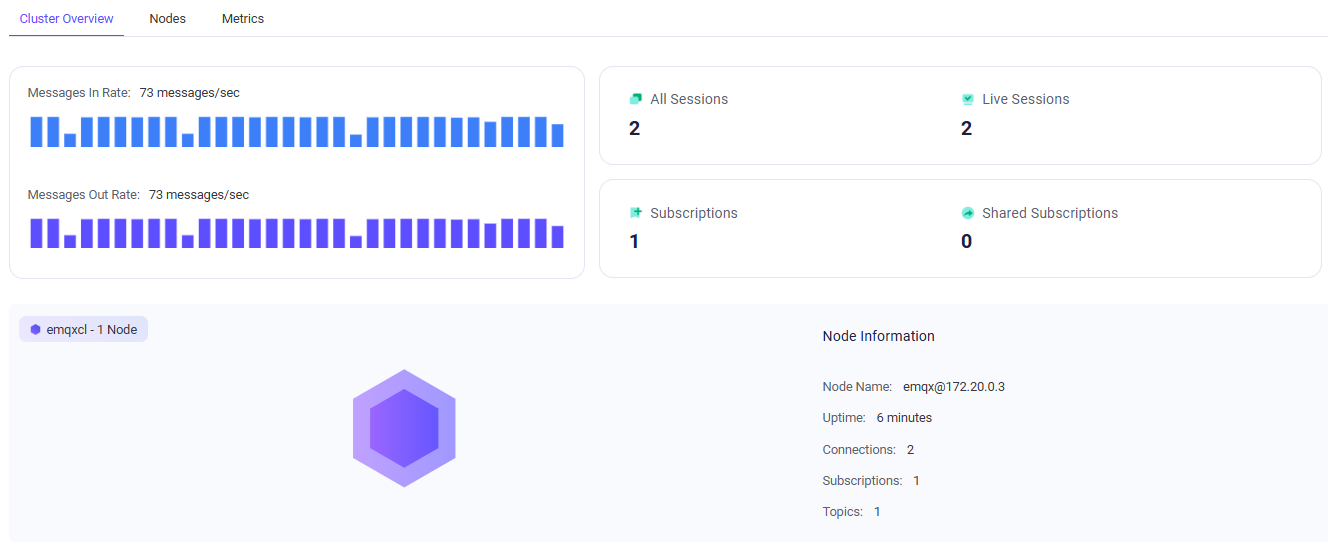
\includegraphics[width=\linewidth]{2 - Ingurunea/emqx.png}
    \caption{EMQX zerbitzariaren \textit{dashboard} nagusia.}
    \label{fig:emqx}
\end{figure}

\subsection{Telegraf eta InfluxDB}
Orduan, sentsoreek MQTT bidez bidalitako mezuak jasotzeko \textit{Telegraf} erabiliko da \cite{noauthor_telegraf_2022}. Honek MQTT harpidedun moduan joka dezake, zerbitzari bateko mezuak jaso eta datu-base batera bidaltzkeo (\textit{InfluxDB}, adibidez). Kode irekiko agente arina da, eta martxan jartzeko TOML moduko konfigurazio artxibo bat baino ez du behar: \textit{telegraf.conf}.\\

Artxibo horretan, lehenik eta behin \textit{agent} atala zehaztu behar da: datuak jasotzeko eta bidaltzeko tarteak, datu \textit{buffer}-aren tamaina, denboraren zehaztasuna... Ondoren, hainbat sarrera (\textit{input}) eta irteera (\textit{output}) plugin zehaztu daitezke; hona hemen sarreran MQTT datuak hartzen dituen eta irteeran \textit{InfluxDB}-ra bidaltzen dituzten pluginen adibideak:\\

\begin{verbatim}
[[inputs.mqtt_consumer]]
  servers = ["tcp://mqtt_broker:1883"]  # MQTT zerbitzariaren helbidea.
  topics = ["sensor/#"]                 # Sensor azpitopic-etara harpidetu.
  qos = 0
  data_format = "json"                  # Datuen formatua.

[[outputs.influxdb_v2]]
  urls = ["http://influxdb_sim:8086"]   # InfluxDB datu-basearen helbidea.
  token = "***"                         # Autentifikazio token-a.
  organization = "gaudee"               # InfluxDB proiektuaren izena.
  bucket = "linac7"                     # Datuak gordetzeko edukiontzia.
\end{verbatim}

Konfigurazioa sinpleagoa eta egonkorragoa izan dadin, zerbitzarien IP helbide zehatzak erabili beharrean, \ref{sec:docker}. atalean azalduko diren \textit{Docker Compose} edukiontzien izenak erabiltzea askoz fidagarriagoa da (\textit{mqtt\_broker}, \textit{influxdb\_sim}). Izen horiek ingurune\hyp{}aldagai moduan jokatzen dute, eta zerbitzuaren sare birtuala martxan jartzean, sortutako IP egokiak automatikoki esleitzen dira, komunikazio\hyp{}arazoak saihestuz.
\newpage
\textit{InfluxDB} denbora-serieak gordetzeko kode irekiko datu-basea da \cite{noauthor_influxdb_2022}. Datu-bolumen handietarako optimizatuta dagoenez, sentsore-datuen biltegiratzerako, kontsultarako eta irudikapenerako aproposa da (\ref{fig:influx_dashboard}. irudia).\\

Denbora-serieak \ref{tab:influxdb}. taulan ikus daitekeen moduan antolatzen dira:

\begin{itemize}
    \item \textbf{Bucket.}  Datuak gordetzeko edukiontzia, hainbat \textit{measurement} izan ditzake.
    \item \textbf{Measurement.} Datu multzoen izena, hainbat \textit{tag} eta \textit{fields} izan ditzake.
    \item \textbf{Tags.} Datuen metadatuen etiketa indexatuak, balioak iragazteko.
    \item \textbf{Fields.} (Giltza, balio) bikoteak, denboran aldatzen diren balioak gordetzeko.
    \item \textbf{Timestamp.} Datu bakoitza denbora zehatz batera lotuta dago.
\end{itemize}

\begin{table}[h]
    \centering
    \begin{tabular}{lllll}
        \toprule
        \textbf{Time} & \textbf{Measurement} & \textbf{Host} & \textbf{Field} & \textbf{Value} \\
        \midrule
        2025-08-18T00:00:00Z & mqtt-consumer & 2b561c0cbef3 & ForwardPower & 80.0739 \\
        2025-08-18T00:00:00Z & mqtt-consumer & 2b561c0cbef3 & ForwardPower & 80.0412 \\
        2025-08-18T00:06:00Z & mqtt-consumer & 2b561c0cbef3 & ForwardPower & 80.1040 \\
        2025-08-18T00:06:00Z & mqtt-consumer & 2b561c0cbef3 & ForwardPower & 79.9736 \\
        \bottomrule
    \end{tabular}
    \caption{\textit{InfluxDB}-n gordetako denbora-serieen adibidea.}
    \label{tab:influxdb}
\end{table}

\begin{figure}[h]
    \centering
    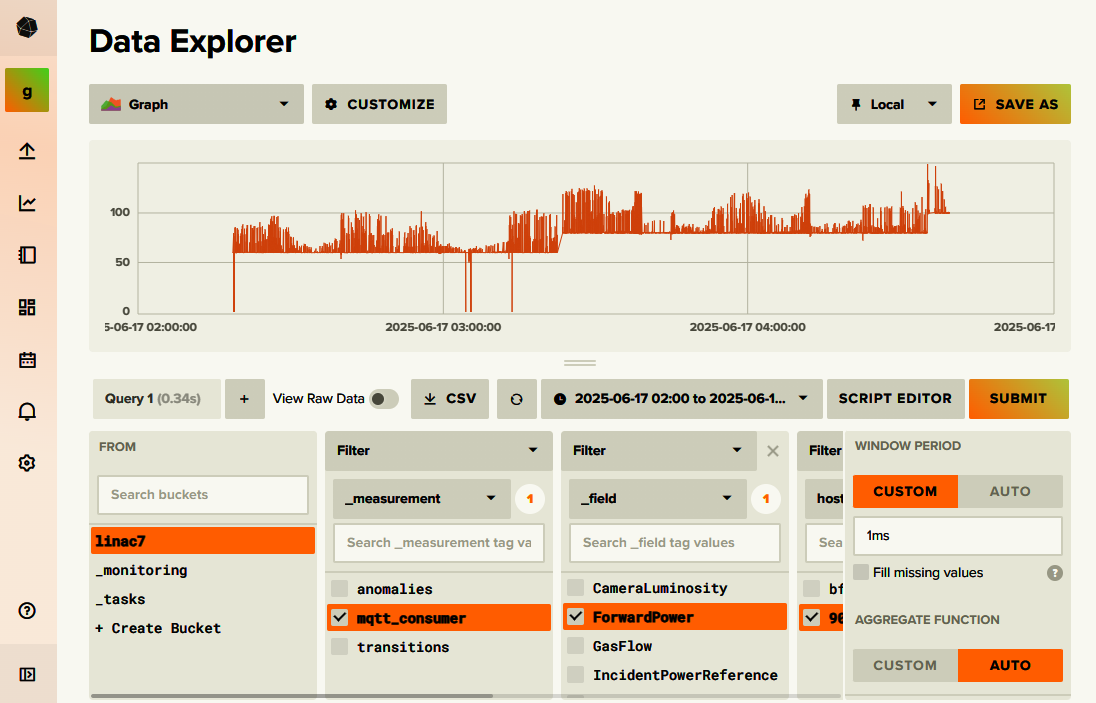
\includegraphics[width=\linewidth]{2 - Ingurunea/influxdb.png}
    \caption{\textit{InfluxDB} datu-basearen kontsulta \textit{dashboard} nagusia.}
    \label{fig:influx_dashboard}
\end{figure}
\newpage
Garatuko diren aplikazioek bertatik jasoko dituzte datuak. Horretarako, kontsulta mekanismo nagusi bat existitzen da \textit{InfluxDB}-n: Flux lengoaia. Honen bidez, denbora\hyp{}serieak erraz iragazi eta eraldatu daitezke. Adibidez, hurrengo kodeak "linac7" \textit{bucket}\hyp{}eko \textit{ForwardPower} magnitudearen azken 50 segunduetako datuak kontsultatzen ditu, denboraren arabera ordenatuta:
\begin{verbatim}
    from(bucket: "linac7")
            |> range(start: -50s)
            |> filter(fn: (r) => r["_measurement"] == "mqtt-consumer")
            |> filter(fn: (r) => r["_field"] == "ForwardPower")
            |> sort(columns: ["_time"])
        '''
\end{verbatim}
\subsection{Docker}
\label{sec:docker}
\textit{Docker} aplikazioak garatzeko, garraiatzeko eta exekutatzeko kode irekiko plataforma da \cite{noauthor_what_2025}. Aplikazioak \textbf{edukiontzi} izeneko ingurune isolatu eta arinetan biltzen dira, exekuziorako beharrezko guztia gordez: fitxategiak, konfigurazioak, liburutegiak... Horrela, edozein sistema eragiletan exekutatu daitezke, bateragarritasun arazoak saihestuz eta makina birtualetan baino baliabide gutxiago erabiliz.\\

Gainera, hainbat aplikazio batera inplementatu daitezke edukiontzi desberdinak erabiliz, eta edukiontzien isolamenduari esker, batek huts egiten badu, ez du besteetan eragiten. Honi \textit{Docker Compose} deritzo, eta oso interesgarria da zerbitzuak garatzeko, aipatutako teknologiak batera inplementatzea ahalbidetzen baitu YAML konfigurazio fitxategi sinple baten bidez (\textit{docker-compose.yml)}. Fitxategi horretan, edukiontzi bakoitza banan-banan definitzen da, eta horren funtzionamendu egokirako ezaugarriak ere:

\begin{verbatim}
services:

    mqtt_broker:
      image: emqx/emqx:5.4.1
      container_name: emqx
      ports:
        - "1883:1883"
        - "18083:18083"
      networks:
        - simulations
\end{verbatim}

\begin{itemize}
    \item \textbf{MQTT zerbitzaria (EMQX)}. Hori definitzeko nahikoa da zerbitzuaren irudia, atakak, sare birtuala eta edukiontziaren izena zehaztea. Kasu honetan bi ataka baino ez dira erabiliko: 1883, MQTT protokolo estandarrerako; eta 18083, \textit{dashboard}-erako.
\end{itemize}
\newpage
\begin{verbatim}
    telegraf:
        image: telegraf:1.30
        container_name: telegraf_sim
        volumes:
          - ./telegraf/telegraf.conf:/etc/telegraf/telegraf.conf:ro
        depends_on:
          - influxdb
          - mqtt_broker
        networks:
          - simulations
        command: ["sh", "-c", "sleep 20 && telegraf"]
\end{verbatim}

\begin{itemize}
    \item \textbf{\textit{Telegraf}}. Konfigurazio fitxategiaren (\textit{telegraf.conf}) helbidea zehaztu behar da; \textit{Read Only} (ro) moduan irekiko da segurtasuna bermatzeko. Gainera, MQTT eta \textit{InfluxDB} erabiltzen dituenez, horiekiko menpekotasuna zehaztu behar da. Azkenik, \textit{sleep 20} komandoa erabiltzen da, EMQX hasieratzea berehalakoa ez denez, horretara konektatzeko 20 segundo itxaron behar baitira.
\end{itemize}

\begin{verbatim}
  influxdb:
    image: influxdb:2.7
    container_name: influxdb_sim
    ports:
      - "8086:8086"
    volumes:
      - influxdb_simulation:/var/lib/influxdb2
    environment:
      - DOCKER_INFLUXDB_INIT_MODE=setup
      - DOCKER_INFLUXDB_INIT_USERNAME=***
      - DOCKER_INFLUXDB_INIT_PASSWORD=***
      - DOCKER_INFLUXDB_INIT_ORG=gaudee
      - DOCKER_INFLUXDB_INIT_BUCKET=linac7
      - DOCKER_INFLUXDB_INIT_ADMIN_TOKEN=***
    networks:
      - simulations
\end{verbatim}

\begin{itemize}
    \item \textbf{\textit{InfluxDB}}. Kasu honetan ere \textit{dashboard}-erako ataka zehaztu behar da, 8086. Horrez gain, datuak gordetzeko bolumena zehaztu behar da. Bestalde, \textit{InfluxDB} hasieratzeko aldagaiak definitu behar dira: erabiltzailea, pasahitza, erakundearen izena, \textit{bucket}-a eta autentifikazio \textit{token}-a.
\end{itemize}

\begin{verbatim}
volumes:
  influxdb_simulation:
networks:
  simulations:
    driver: bridge
\end{verbatim}

Azkenik, \textbf{datu-bolumenak} eta \textbf{sare birtuala} definitzen dira: bolumenari esker, nahiz eta zerbitzua itzali, bertako datuak mantenduko dira; eta sareak, ordea, edukiontzien arteko komunikazioa ahalbidetzen du, ingurune-aldagaiak eta IP helbideak partekatuz.\\

Bestalde, Python \textit{script}-ak edukiontzietan inplementatu daitezke ere. Horretarako, bi fitxategi laguntzaile behar dira. Alde batetik, \textit{requirements.txt}, programak funtzionatzeko beharrezkoak diren liburutegien zerrenda; adibidez:

\begin{Verbatim}[fontsize=\footnotesize]
    pandas
    paho-mqtt
    numpy
    scipy  
\end{Verbatim}

Bestetik, edukiontziaren eraikuntza definitzen duen fitxategia, \textit{Dockerfile}:

\begin{Verbatim}[fontsize=\footnotesize]
    FROM python:3.9-slim-buster

    # Kontenedorean lan-helbidea definitu
    WORKDIR /app
    # Kopiatu kontenedorean instalatu beharreko moduluak dituen testu fitxategia
    COPY requirements.txt requirements.txt
    # Instalatu moduluak
    RUN pip install -r requirements.txt
    # Kopiatu programa kontenedorean
    COPY simulator.py simulator.py

    # Exekutatu
    CMD ["python", "simulator.py"]
\end{Verbatim}

Horiek sortuta, \textit{Docker Compose}-aren barruan integratu daiteke, beste edukiontziekin automatikoki exekutatzeko, eta horien arteko menpekotasun eta ingurune-aldagaiak erraz definitzeko. \textit{docker-compose.yml} fitxategian gehitu beharreko kodearen adibidea, EMQX hasieratzeko eta horretara konektatzeko itxaron-denbora kontuan hartuta (\textit{sleep 20} komandoa):

\begin{Verbatim}[fontsize=\footnotesize]
    services:
      simulator:
        build:
          context: simulator
          dockerfile: Dockerfile
        container_name: simulator
        volumes:
          - ./data:/app/data
        depends_on:
          - mqtt_broker
        environment:
          MQTT_BROKER_HOST: mqtt_broker
          MQTT_TOPIC: data
        networks:
          - simulations
        command: ["sh", "-c", "sleep 20 && python simulator.py"]
\end{Verbatim}

Orduan, zerbitzua gordeko den karpetan \textit{docker-compose.yml} fitxategia izanik, eta \textit{telegraf} azpikarpetan \textit{telegraf.conf} fitxategia izanik, beste aplikazioek konfigurazio gehiagorik behar ez dutenez, nahikoa da ordenagailuaren kontsolan karpeta nagusira joan eta hurrengo komandoa exekutatzea:

\begin{Verbatim}
    docker compose up -d
\end{Verbatim}

Horrela, aplikazio guztiak atzeko planoan (\textit{-d}) exekutatuko dira, bakoitza bere edukiontzian, eta monitorizazioa kontsolatik edo \textit{Docker Desktop} aplikaziotik egin daiteke. Azken honek edukiontzien egoera, \textit{log}-ak eta errendimendua ikustarazteko interfaze grafiko bat eskaintzen du (\ref{fig:docker-desktop}. irudia).\\

\begin{figure}[h]
    \centering
    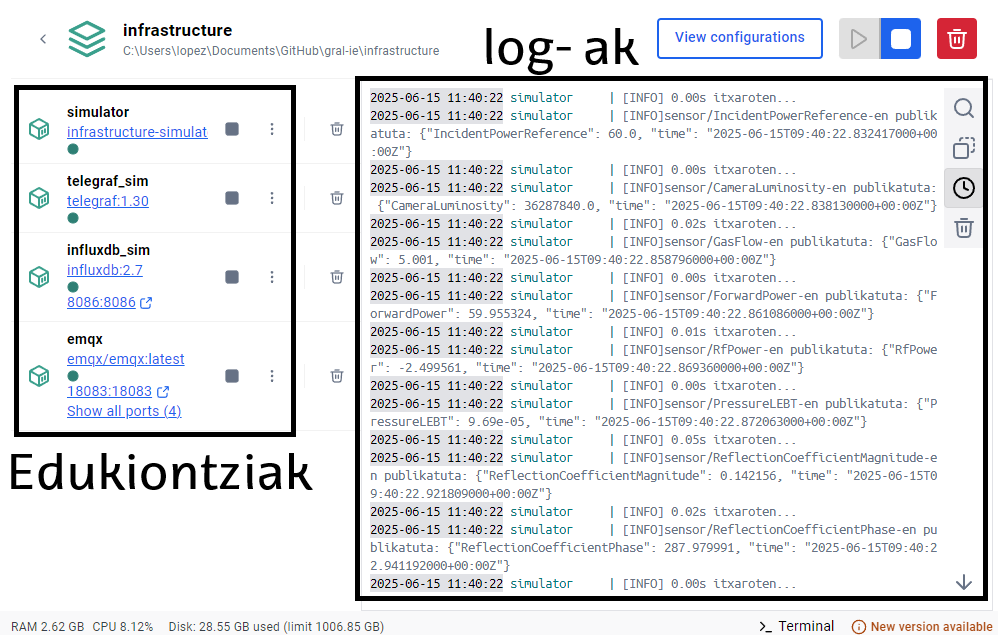
\includegraphics[width=\linewidth]{2 - Ingurunea/docker-desktop.png}
    \caption{\textit{Docker Desktop} aplikazioaren interfazea, edukiontziak eta \textit{log}-ak.}
    \label{fig:docker-desktop}
\end{figure}

Azkenik, sistemaren exekuzioa amaitzeko, hurrengo komandoa erabiltzen da:

\begin{Verbatim}
    docker compose down
\end{Verbatim}

Honen bidez zerbitzua gelditu eta edukiontziak ezabatzen dira, baina bolumenetako datuak (\textit{influxdb\_simulation}) mantenduz.
\newpage
\section{Neurketak}
\ref{sec:ez-intrusibo} atalean aipatu den moduan, detektoreetako eta kamerako informazioa sare-lokalera konektatutako edozein ordenagailutan jaso daiteke. Horrez gainera, gas-kontroladorearen gas-fluxua eta RF sorgailuaren potentzia eta maiztasuna alda daitezke ere. Atal honetan jasotako magnitudeetan eta aldagaietan sakonduko da.\\

Dena dela, sistema probatzeko saiakera batean egindako akatsen ondorioz, eremu magnetikoa sortzen duten iman iraunkorrak erabilgaitz bilakatu dira testu hau idatzitako unean, eta plasma sortzea ezinezkoa denez, neurketa berriak lortzea ere ezinezkoa izan da. Hori dela eta, akats eta trantsizioen detekzio-zerbitzua garatzeko eta probatzeko aurreko saiakeren datu historikoak erabili dira.

\subsection{Aldagaiak eta magnitudeak}

PIT30 ioi-iturrian egindako neurketetan, RF sorgailuaren maiztasuna konstante mantendu da, 3 GHz-ko maiztasunean erresonatzeko diseinatuta dagoelako. Hala ere, 2.993 GHz-tan erresonantzia hobea behatu denez, hori finkatu da. Beraz, eskuz aldatu daitezkeen bi parametro daude ganberaren portamoldea aldatzeko:

\begin{itemize}
    \item \textbf{RF sorgailuaren potentzia.} Sortutako seinalearen potentzia dBm-tan adierazten da: gehienez 0 dBm-koa da (1 mW), baina ondoren, seinalea irabazi finkoko anplifikadore batekin 500 W-eraino anplifikatu daiteke.
    \item \textbf{Gas-fluxua.} Gas-kontroladoreak sccm-tan (\textit{Standard Cubic Centimetres per Minute})
    ezartzen du tenperaturaren independenteki: gehienez 5 sccm ezarri daitezke.
\end{itemize}

Bestalde, aldagai horiek aldatuz, betiere zarata saihesteko plasmaren egonkortze-denbora errespetatuz, potentzia-detektoreek eta kamerak emandako informazioarekin hurrengo magnitudeak erabili dira diagnostikorako:

\begin{itemize}
    \item \textbf{Argitasuna}. Kameraren pixel guztien argitasunen batura, erreferentzia balio batekiko unitate arbitrariotan (\textit{a.u.}) emanda. Kameraren kokapen eta lerrokatzearen menpekoa denez, neurketak kalibratuta egotea funtsezkoa da. 
    \item \textbf{Aurreranzko potentzia.} Potentzia detektoreak neurtutako aurreranzko seinalearen potentzia, watt-etan (\textit{W}) emanda. Detektorean tentsio diferentzia bezala neurtzen da, baina bihurketa baten bidez potentzia lortzen da \cite{noauthor_schottky_2025}.
    \item \textbf{Aurreranzko potentziaren erreferentzia.} RF sorgailura sartu baino lehen eskuz zehaztutako aurreranzko-potentzia, watt-etan (\textit{W}) emanda. Erreferentziazko eta detektorean neurtutakoaren arteko diferentzia \textbf{aurreranzko zarata} kalkulatzeko erabiltzen da.
    \item \textbf{Islapen-koefizientearen magnitudea.} Aurreranzko seinalearen eta islatutako seinalearen potentziaren magnitudearen arteko zatidura. Horrela, aurreranzko potentzia erabiliz, islatutako potentzia lor daiteke.
    \item \textbf{Islapen-koefizientearen fasea.} Aurreranzko seinalearen eta islatutako seinalearen arteko desfasea, graduetan emanda.
    \item \textbf{LEBT-eko presioa.} LEBT-eko gurutzean neurtutako presioa, pascal-etan (\textit{Pa}). Azeleragailuan hutsa beharrezkoa da, eta ioi-iturrian sartutako gas-fluxuaren arabera presioa aldatzen denez, neurtzea beharrezkoa da.
\end{itemize}

Plasmaren diagnostikoan oso garrantzitsua den beste magnitude bat existitzen da ere: \textbf{adaptazioa}, aurreranzko eta islatutako seinaleen potentzien arteko diferentzia; izan ere, erresonantzia ziklotronikoan elektroiek energia potentziatik xurgatzen dutenez, trantsizioetan adaptazioaren aldaketak ikus daitezke. Hortaz, argitasunaren eta adaptazioaren arteko korrelazioa aztertu da \cite{fernandez_rua_clasificacion_2024}:

\begin{table}[h]
    \centering
    \begin{tabular}{c|c|c|c}
         & Argitasuna & Aurreranzko zarata & Adaptazioa \\
         \midrule
         Argitasuna & 1.00 & -0.17 & 0.67\\
         \midrule
         Aurreranzko zarata & -0.17 & 1.00 & -0.11 \\
         \midrule
         Adaptazioa & 0.67 & -0.11 & 1.00 \\
    \end{tabular}
    \caption{Argitasunaren, adaptazioaren eta aurreranzko zarataren korrelazio-matrizea.}
    \label{tab:korrelazioa}
\end{table}

Beraz, argitasunean behatutako aldaketak adaptazioa soilik erabiliz detekta daitezke, baina korrelazioa behar bezain altua ez denez ($\approx0.67$), saltoak egoki identifikatzeko beste magnitude bat gehitzea beharrezkoa da: \textbf{aurreranzko zarata}.\\

Trantsizioak detektatzeko, gas-ekorketak erabili dira; hau da, RF sorgailuan potentzia bat finkatuz, gas-kontroladorearen fluxua aldatzea, 5 sccm-tik 2 sccm-rako bi ziklo oso eginez. Ekorketa horietan argitasunean trantsizioak behatzea lortu da, eta baita jauzi handiak plasma pizten denean, gas-fluxu minimoetan (\ref{fig:gas-ekorketa60w}. irudia).

\begin{figure}[h]
    \centering
    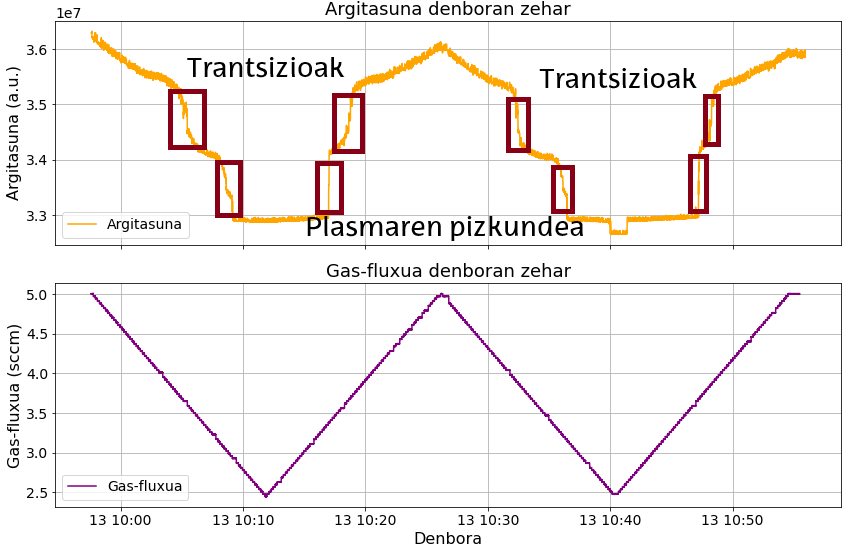
\includegraphics[width=0.9\linewidth]{3 - Neurketak/gas-ekorketa_60w.png}
    \caption{Argitasuna denboran zehar gas-ekorketa baterako, aurreranzko potentziaren erreferentzia 60 W-etan finkatuz.}
    \label{fig:gas-ekorketa60w}
\end{figure}

Azkenik, sentsoreen akatsak detektatzeko daturik existitzen ez denez, datu historikoak eskuz aldatzea erabaki da. Magnitude guztietarako hainbat datu ausaz aldatu dira, balioak handituz, txikituz edo zerora eramanez, horrela sentsoreen disfuntzioak simulatzeko asmoz. Dena dela, akatsak adierazteko metodo honek ez ditu benetako sentsoreen ezaugarriak islatzen, baina zerbitzuaren hasierako entrenamenduetarako erabilgarria da (\ref{fig:gas-ekorketa-akatsa}. irudia).

\begin{figure}[h]
    \centering
    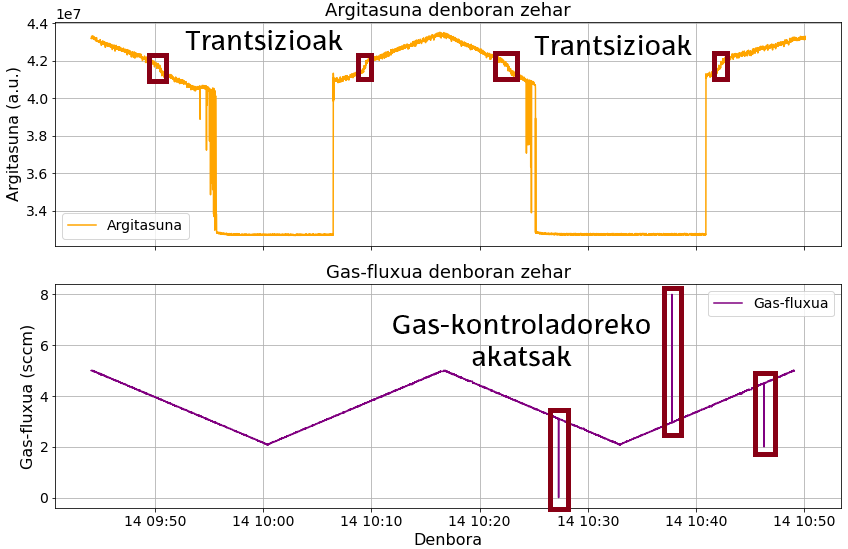
\includegraphics[width=0.8\linewidth]{3 - Neurketak/gas-ekorketa_akatsahutsa.png}
    \caption{Gas-kontroladorearen akatsaren adibidea, hainbat balio eskuz aldatuz.}
    \label{fig:gas-ekorketa-akatsa}
\end{figure}

\subsection{Datu-eskuratze simulazio sistema}
Garatuko den zerbitzuan trantsizioak eta akatsak zuzenean detektatu nahi direnez, zuzeneko datu\hyp{}eskuratzea simulatzeko sistema bat garatu da plasma sortzea ezinezkoa den bitartean, eta \ref{sec:ingurunea}. atalean azaldutako azpiegituran integratu da.

\begin{enumerate}
    \item Lehenik eta behin, \textit{data} karpetako azpikarpetetan gordetako \textit{.csv} fitxategiak irakurtzen dira, ioi-iturriaren gas-ekorketetarako neurtutako magnitudeen informazioa gordetzen dutenak. \textit{Pandas} liburutegiako \textit{DataFrame} bat eraikitzen da sentsore bakoitzerako, eta gordetako denboraren arabera ordenatzen dira.
    \item Ondoren, \textit{paho.mqtt} liburutegiaren bidez MQTT bezero bat sortzen da, eta \textit{docker-compose.yml} fitxategian definitutako ingurune-aldagai baten bidez EMQX zerbitzarira konektatzen da.
    \item Orduan, sentsore guztien arteko denbora-etiketa txikiena bilatzen da, eta magnitude guztien arteko denbora-erlatiboak mantentzen saiatuz, \textit{sensor} \textit{topic}-ean argitaratzen dira, sentsore bakoitzerako azpitopic bat sortuz.
    \item Azkenik, azpikarpeta bateko datu guztiak bidali direnean, eskuz zehaztutako denbora-tarte bat itxaroten da, eta prozesua beste azpikarpetetarako errepikatzen da segidan.
\end{enumerate}

Script-a azpiegituraren barruan integratu da \textit{Docker Compose}-en bidez, \textit{requirements.txt} eta \textit{Dockerfile} fitxategien bidez edukiontzi berri bat definituz; izan ere, \ref{sec:docker}. atalean aipatutako adibideak simulatzaile honetarako fitxategiak dira. Horrela, zuzeneko datuen MQTT bidezko argitalpena simulatzea lortu da, eta baita horien jasotzea \textit{Telegraf}-en bidez, eta biltegiratzea eta ikustaraztea \textit{InfluxDB}-ko \textit{dashboard}-en bidez (\ref{fig:simulator_dashboard}. irudia).

\begin{figure}[h]
    \centering
    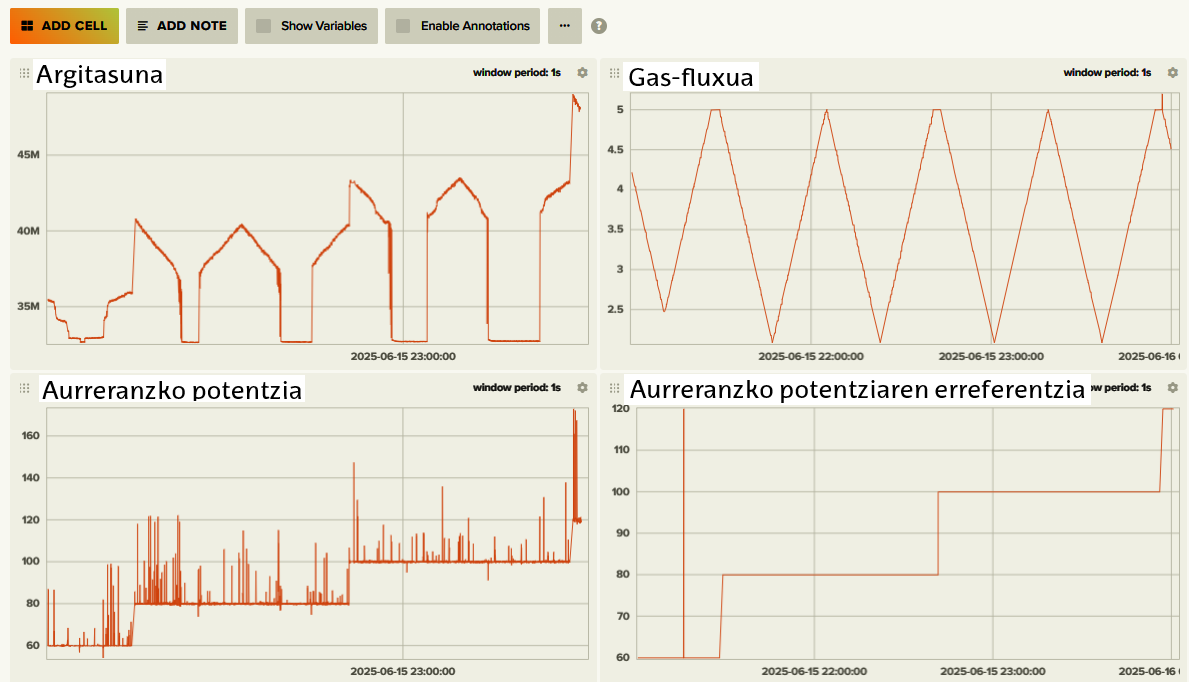
\includegraphics[width=0.92\linewidth]{3 - Neurketak/simulator_dashboard.png}
    \caption{Simulatzaileak argitaratutako magnitudeen \textit{InfluxDB}-ko \textit{dashboard}-a.}
    \label{fig:simulator_dashboard}
\end{figure}

Gainera, simulatzailea guztiz eskalagarria eta orokorra da, azpikarpeta bateko \textit{.csv} fitxategiak irakurtzen baino ez dituelako, eta fitxategiaren izenaren araberako \textit{topic} batean argitaratzen direlako; hau da, magnitude berriak inplementatu nahi izanez gero, nahikoa da horren denboraren araberako datu-fitxategia azpikarpetan gordetzea (\ref{fig:data_magnitude}. irudia). Bestalde, sentsoreen akatsak inplementatzea oso erraza da ere, \textit{.csv} fitxategietako datuak eskuz aldatzea nahikoa baita.\\

Azkenik, ioi-iturria martxan jarri gabe eta sare-lokalera konektatu gabe horren portamoldea simulatu daitekeela da aplikazioaren abantailarik garrantzitsuena. Horrela, iturriaren funtzionamendua edozein tokitik aztertu daiteke, eta baita arazo fisikoak izanda ere, datu historikoei esker.

\begin{figure}[h]
    \centering
    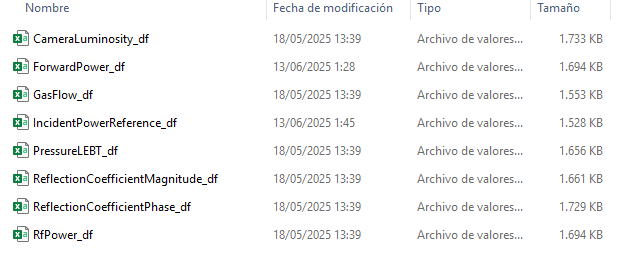
\includegraphics[width=0.65\linewidth]{3 - Neurketak/data_magnitudeak.png}
    \caption{\textit{data} karpetako azpikarpeta baten \textit{.csv} fitxategien adibidea.}
    \label{fig:data_magnitude}
\end{figure}
\newpage
\section{Detekzio teknikak}
\label{sec:teknikak}
Atal honetan, plasma-trantsizioak eta sentsoreen akatsak detektatzeko erabiliko diren tekniketan sakonduko da, aplikazioak garatu baino lehen. Lehenik, trantsizioak detektatzeko, Linac-7 proiektuan garatutako beste lan batean erabilitako metodoa errepikatuko da \cite{fernandez_rua_clasificacion_2024}, baina zuzeneko datuen leihoak hartuz: \textbf{adaptazioaren erregresio-lineala eta aurreranzko zarataren maximoak}. Bestalde, sentsoreen akatsak detektatzeko, \textbf{DBSCAN} klusterizazio algoritmoa erabiliko da: honek datuak dentsitatearen arabera taldekatzen ditu, eta multzo horietatik urruntzen diren datuak anomaliatzat hartzen dira.

\subsection{Trantsizio detekzioa: linregress + find\_peaks }
\label{sec:linregress}

Argitasunean salto bat ematen denean, adaptazioan ere ematen da, eta gainera, aurreranzko zaratak gorakada bat jasaten du (\ref{fig:transitions_luminosity_adaptation}. irudia). Ondorioz, horiek antzemateko metodo intuitibo bat adaptazioaren denborarekiko joera aztertzea izan daiteke, erregresio linealaren bidez malda lortuz. Beraz, salto bat detektatzeko bi baldintza zehaztuko dira:

\begin{itemize}
    \item Adaptazioaren erregresioaren maldak zehaztutako atari-balio bat gainditzea.
    \item Aurreranzko zarataren gorakada inguruko puntuekiko nabarmena izatea, atari-balio bat zehaztuz ere.
\end{itemize}

\begin{figure}[h]
    \centering
    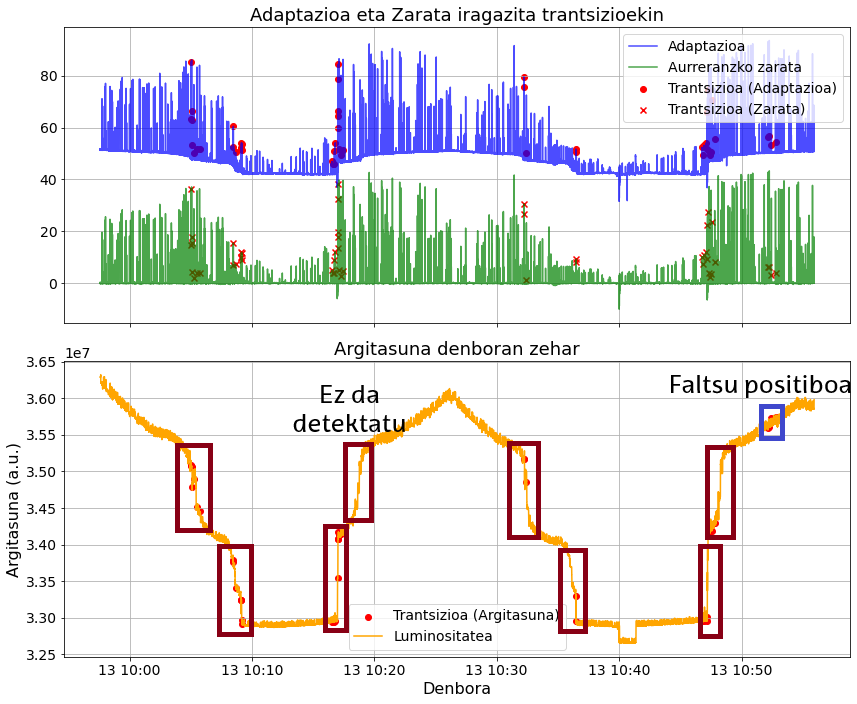
\includegraphics[width=0.8\linewidth]{4 - Detekzio teknikak/argitasuna_adaptazioa_saltoak.png}
    \caption{Argitasunean eta adaptazioan behatutako trantsizioak eta horien identifikazio automatikoa.}
    \label{fig:transitions_luminosity_adaptation}
\end{figure}

Horretarako, bi funtzioak inplementatzen dituen liburutegi apropos bat existitzen da Python-en: \textit{scipy} \cite{scipy_scipystats_2025}. Honek \textit{linregress} funtzioa barneratzen du, bi datu multzoetarako karratu-minimoen erregresio lineala kalkulatzen duena, eta baita \textit{find\_peaks} ere, seinale baten gailurrak topatzeko.

\paragraph{linregress} \leavevmode\\

Funtzio honek luzera berdina (N) duten bi datu multzo (x, y) hartu eta horien arteko erlazio lineala deskribatzen duen lerro zuzen egokiena kalkulatzen du (\ref{fig:linear_regression}. irudia), eta horren malda eta abzisa-ebakidura bueltatzen ditu \cite{scipy_scipystats_2025}:

\begin{equation}
    y = malda \cdot x + ebakidura
\end{equation}

Horretarako, \textbf{karratu-minimoen metodoaz} baliatzen da. Horren arabera, erregresioak emandako eta benetako balioen arteko diferentzia minimizatzeko, lerro zuzen egokienaren malda xy-ren kobariantzaren eta x-ren bariantzaren arteko zatidura da:

\begin{equation}
    \begin{aligned}
        SS_{xy} &= \sum (x_i - \bar{x})(y_i - \bar{y})\\
        SS_{xx} &= \sum (x_i-\bar{x})^2 \\
    \end{aligned}
    \quad
    \Longrightarrow
    \quad
    malda = \frac{SS_{xy}}{SS_{xx}}
\end{equation}\\
non $\bar{x},\bar{y}$ emandako multzoen bi magnitudeen batezbesteko balioak diren. Horiek kalkulatzeko, eta baita kobariantza eta bariantza kalkulatzeko, \textit{numpy} liburutegia erabiltzen da. Abzisa-ebakidura, ordea, maldaz baliatuz lortu daiteke, lerro zuzena bi datuen batezbesteko puntutik igarotzen baita:

\begin{equation}
    ebakidura = \bar{y}-malda \cdot \bar{x}
\end{equation}

Beraz, praktikan bi balio horiek lortzeko, nahikoa da \textit{linregress} funtzioa honela deitzea:

\begin{verbatim}
    malda, ebakidura, _, _, _ = linregress(x, y)
\end{verbatim}

Kasu honetan, x-multzoa denbora izango da, eta y-multzoa, berriz, seinalearen potentziaren adaptazioa.

\begin{figure}[h]
    \centering
    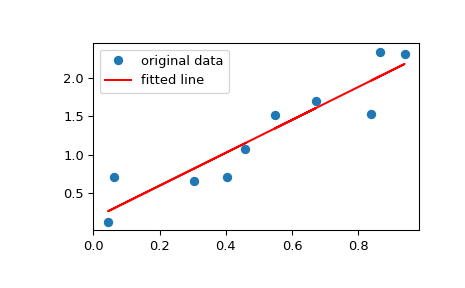
\includegraphics[width=0.55\linewidth]{4 - Detekzio teknikak/linear_regression.png}
    \caption{Erregresio lineal baten adibide sinplea.}
    \label{fig:linear_regression}
\end{figure}

\paragraph{find\_peaks} \leavevmode\\

Funtzio honek dimentsio bakarreko datu-multzo baten maximo lokalak aurkitzen ditu, ondoz-ondoko puntuen hainbat propietate konparatuz: altuera, zabalera, puntuen arteko distantzia, prominentzia... Hala ere, kasu honetan gailurrak identifikatzeko prominentzia (\textit{prominence}) baino ez da erabiliko (\ref{fig:prominence}. irudia).

\begin{figure}[h]
    \centering
    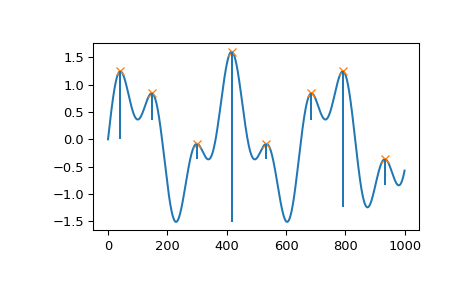
\includegraphics[width=0.55\linewidth]{4 - Detekzio teknikak/prominences.png}
    \caption{Seinale baten maximoen prominentziaren kalkuluaren adibide sinplea.}
    \label{fig:prominence}
\end{figure}

Gailur baten \textbf{prominentziak} bere inguruko puntuekiko zenbat gailentzen den kuantifikatzen du \cite{scipy_scipysignal_2025}. Horretarako, maximoetatik ezker eta eskuinerako puntuak zeharkatzen dira maximo altuago bat aurkitu arte, eta bi tarte horietarako balio minimoak bilatzen dira. Bi minimo horiei \textbf{gailurraren oinarri} deritze, eta handiena hartuz, gailurraren balioaren eta oinarriaren arteko diferentzia da prominentzia.\\

Praktikan gailurrak lortzeko, nahikoa da \textit{find\_peaks} funtzioa honela deitzea, \textit{prominence} balioa eskuz aukeratuz:

\begin{verbatim}
    index, _ = find_peaks(df["NoiseForward"], prominence=prominence_noise)
\end{verbatim}

Kasu honetan, aurreranzko seinalearen zarataren maximoak bilatuko dira, eta prominentziaren balioa zehazteko probak hurrengo atalean azalduko dira.

\paragraph{EWMA iragazketa} \leavevmode\\

Sentsoreen bidez lortutako magnitudeek zarata nabarmena dute, eta  horrek erregresio-lineala kalkulatzerakoan edo maximoak bilatzerakoan eragin nabarmena izan dezake. Hori dela eta, gomendagarria da funtzio horiek aplikatu baino lehen magnitudeak iragaztea, seinalearen joera orokorra hobeto antzemateko.\\

ECR motako ioi-iturrien magnitudeen prozesaketan hainbat teknika desberdin erabili daitezke \cite{wang_ion_2024} \cite{rajagopalan_generalized_2003}. Kasu honetan EWMA (\textit{Exponentially Weighted Moving Average}) iragazkia aukeratu da \cite{ross_chapter_2021}, horren inplementazioa oso erraza delako: \textit{pandas} liburutegiak datu-multzo batean iragazki hori aplikatzen duen funtzioa barneratzen du (\textit{DataFrame.ewm}).\\

Iragazki honetan, momentuko magnitudearen ($x_t$) leundutako balioa kalkulatzeko ($\omega_t$) aurreko balioa erabiltzen da ($\omega_{t-1}$), momentuko balioa $\alpha \in [0,1]$ pisuarekin biderkatuz, eta aurrekoa ($1-\alpha$) pisuarekin:\\

\begin{equation}
    \omega_t = \alpha \cdot x_t + (1-\alpha) \cdot \omega_{t-1}
\end{equation}\\

Funtzioa errekurtsiboa denez, aurreko balioak ($1-\alpha$) faktoreaz esponentzialki biderkatzen dira, eta horrela, iraganeko balioen eragina denborarekin azkar murrizten da, balio berrienei garrantzia handiagoa emanez. Hortaz, \textbf{$\mathbf{\alpha}$ parametroa doituz} iragazkiaren erantzuna kontrola daiteke: balio handiagoetarako leundutakoa momentukoaren antzekoagoa izango da, eta erantzuna azkarragoa; eta balio txikiagoetarako, berriz, seinalea leunagoa izango da, baina erantzuna motelagoa. Hau da, mota honetako iragazkiek $\alpha$ balioaren araberakoa atzerapen bat sartzen dute (\ref{fig:ewma_example}. irudia).\\

\begin{figure}[h]
    \centering
    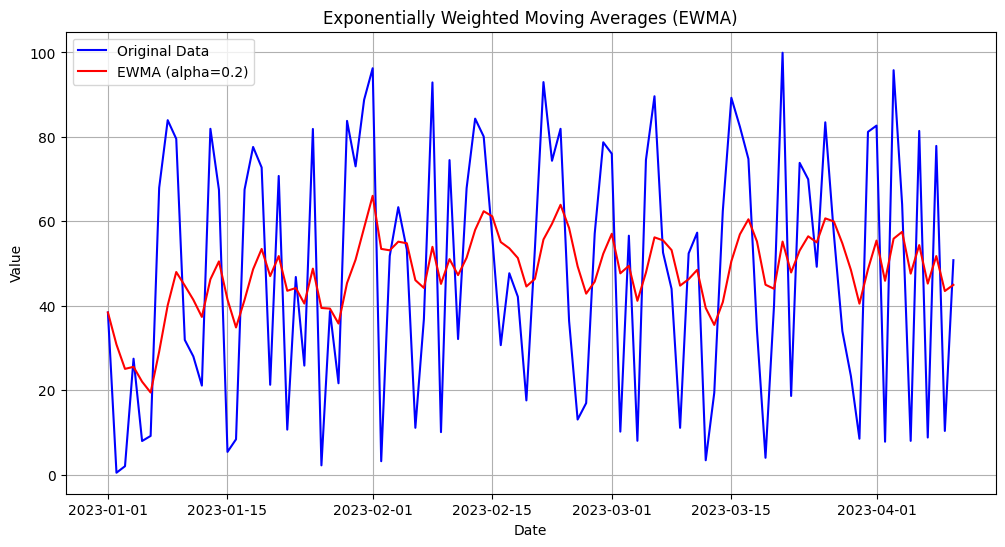
\includegraphics[width=0.9\linewidth]{4 - Detekzio teknikak/ewma_example.png}
    \caption{EWMA iragazketaren adibide sinplea eta atzerapena ($\alpha = 0.2$).}
    \label{fig:ewma_example}
\end{figure}

\subsection{Akatsen detekzioa: DBSCAN}
\label{sec:dbscan}
DBSCAN (\textit{Density Based Spatial Clustering of Applications with Noise}) \cite{ester_density-based_1996} datuak dentsitatearen arabera multzokatzeko \textit{clustering} algoritmoa da, datuen arteko distantzia kontuan hartuta. Horretarako, bi aldagai baino ez dira definitu behar:

\begin{itemize}
    \item $\mathbf{\epsilon}$ \textbf{(epsilon)}. Puntu batetik beste puntu bat auzokotzat hartzeko distantzia maximoa.
    \item \textbf{minPts.} Puntu bat multzo berri baten nukleotzat hartzeko bere inguruan $\epsilon$ distantziara egon beharreko puntu minimo kopurua.
\end{itemize}

Hori kontuan hartuta, hiru motako puntuak bereiz daitezke algoritmoan (\ref{fig:dbscan_points}. irudia):

\begin{itemize}
    \item \textbf{Nukleo-puntuak} (\textit{core-points}). Horren inguruan gutxienez \textit{minPts} puntu $\epsilon$ distantzia edo txikiagora dituztenak. Inguruko puntu horiei \textbf{zuzeneko-irisgarri} (\textit{directly reachable}) deritze.
    \item \textbf{Puntu-irisgarriak} (\textit{reachable-points}). Nukleo-puntu batetik zuzeneko-irisgarriak direnak ($\epsilon$ distantziara), baina horien inguruan \textit{minPts} puntu ez dituztenak.
    \item \textbf{Anomaliak}. Edozein puntutik irisgarriak ez direnak.
\end{itemize}

\begin{figure}[h]
    \centering
    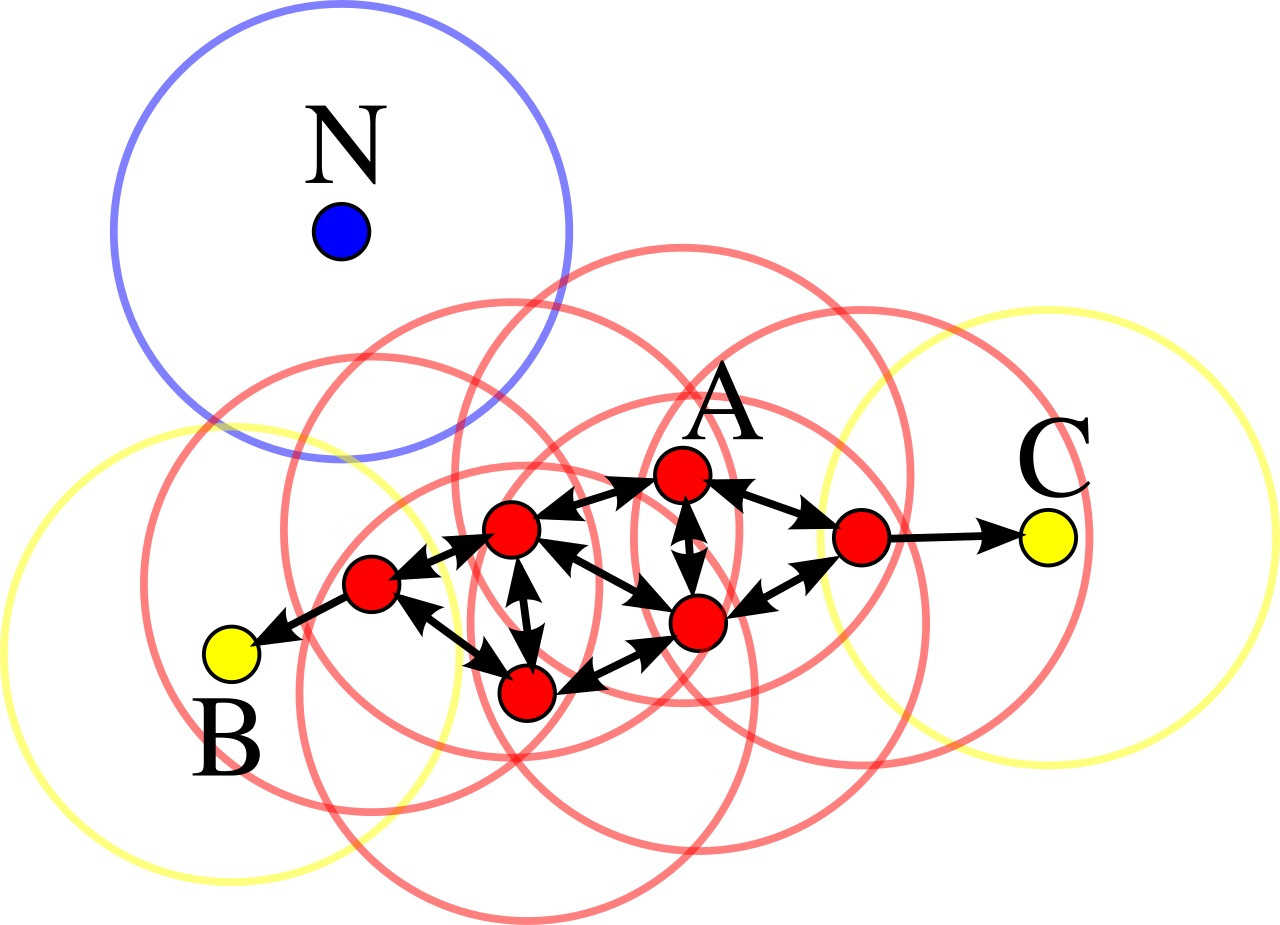
\includegraphics[width=0.4\linewidth]{4 - Detekzio teknikak/DBSCAN-Illustration.jpg}
    \caption{DBSCAN-en puntuen irudikapena. Kasu honetan, A puntua nukleoa da; B eta C beste nukleoetatik irisgarriak dira; eta azkenik, N anomalia bat da.}
    \label{fig:dbscan_points}
\end{figure}

Beraz, puntu multzoak naturalki identifikatzeko gai da DBSCAN, \textit{cluster} kopurua aldez aurretik definitu gabe, eta anomaliak dentsitate-baxuaren arabera detektatzen dira. Horregatik, oso erabilia da sentsoreen akatsen identifikazioan \cite{doreswamy_fault_2014}.\\


Praktikan, algoritmoa inplementatzeko liburutegi bat existitzen da Python-en: \textit{scikit-learn} \cite{scikit-learn_dbscan_2025}. Honek \textit{DBSCAN} funtzioa barneratzen du, eta \textit{eps} eta \textit{min\_samples} aldagaiak eskuz aukeratuz, datu-multzo bateko (X) anomaliak honela lortu daitezke (\ref{fig:dbscan_anomaliak}. irudia):

\begin{verbatim}
    clustering = DBSCAN(eps=eps, min_samples=min_samples).fit(X)
    clustering.labels_ # Etiketetan -1 duten puntuak anomaliak dira
\end{verbatim}

Algoritmoaren eraginkortasuna \textit{eps} aldagaiaren aukeraketan oinarritzen da batez ere. Ondorioz, datu-multzoaren dimentsioa handitu ahala, puntuen arteko distantzia horren aukeraketa zaila izan daiteke, eta gomendagarria da dimentsio baxutan lan egitea. Bestalde, puntuen arteko distantzia kalkulatzeko, \textit{scikit-learn} liburutegiko funtzioan Minkowski metrikaren dimentsioaren balioa (\textit{p}) zehaztu daiteke ere, baina defektuz p=2 erabiltzen da, distantzia Euklidearra:

\begin{equation}
    d (p,q) = \sqrt{\sum_{i=1}^n |p_i - q_i|^2}
\end{equation}
\newpage
\begin{figure}[h]
    \centering
    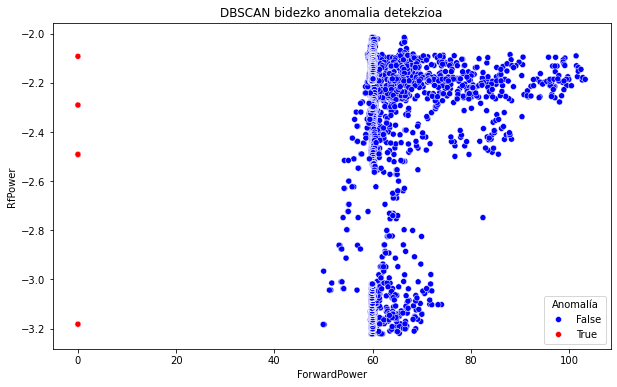
\includegraphics[width=\linewidth]{4 - Detekzio teknikak/dbscan_anomaliak.png}
    \caption{RF sorgailuko magnitudeen DBSCAN anomalia detekzioaren adibidea.}
    \label{fig:dbscan_anomaliak}
\end{figure}

\newpage
\section{Zerbitzuaren garapena eta funtzionamendua}
Azkenik, trantsizioak eta akatsak detektatzeko aplikazioen garapena azalduko da. Aurreko ataletan deskribatutako azpiegiturak erabiliz, \textit{Docker}-eko bi edukiontzi berri sortu dira, \textit{InfluxDB} periodikoki kontsultatzen dutenak eta datuak Python-en bidez prozesatzen dituztenak, azaldutako tekniketan oinarrituta. Honelakoa da aplikazioen egitura:

\begin{multicols}{2}
\begin{verbatim}
Trantsizio-detekzioa
 - Dockerfile
 - requirements.txt
 - transitions.py
\end{verbatim}

\columnbreak

\begin{verbatim}
Akats-detekzioa
 - Dockerfile
 - requirements.txt
 - faults.py
\end{verbatim}
\end{multicols}

Lehenik eta behin, script-ek erabiliko dituzten liburutegiak inportatzea ezinbestekoa da. Programak \textit{Docker} ingurunean exekutatuko direnez, liburutegi horiek \textit{requirements.txt} fitxategian zehaztu behar dira. Detekzioetarako \ref{sec:teknikak}. atalean azaldutako funtzioak erabiliko direnez, hauek dira erabiliko diren liburutegiak:\\

\begin{verbatim}
    pandas            # Datuak DataFrame-etan antolatu eta EWMA iragazkia
    numpy             # Datuen tratamendua
    influxdb-client   # InfluxDB-ra konektatu eta datuak kontsultatu
    scipy             # linregress eta find_peaks funtzioak
    scikit-learn      # DBSCAN funztioa
\end{verbatim}

Orduan, datuak kontsultatzeko \textit{InfluxDB} bezero bat hasieratzen da programa bakoitzean, \textit{.env} fitxategian definitutako ingurune-aldagaiak erabiliz. Horrela, bezeroaren konfigurazioa aldatzea erraza da, \textit{docker-compose.yml} konfigurazio fitxategiak edo script-ak aldatu behar gabe:\\

\begin{verbatim}
    INFLUX_URL=http://***:8086
    INFLUX_TOKEN=***
    ORGANIZATION=gaudee
    BUCKET=linac7
\end{verbatim}

\subsection{Trantsizio detekzioa}

Trantsizioak detektatzeko adaptazioa eta aurreranzko zarata baino ez direnez behar, \textit{get\_data} funtzioaren bidez azken 50 segundoetako \textit{Aurreranzko potentzia}, \textit{Aurreranzko potentziaren erreferentzia} eta \textit{Islapen-koefizientearen magnitudea} kontsultatzen dira, eta denboraren arabera ordenatutako \textit{pandas} DataFrame-ak sortzen dira magnitude bakoitzerako. Gainera, trantsizioen detekzioa ziurtatzeko, \textit{get\_data} funtzioa 5 \textbf{segundoero} deitzen da, datuen gainezarmena bermatuz.

\begin{verbatim}
    from(bucket: "{bucket}")
            |> range(start: -50s)
            |> filter(fn: (r) => r["_measurement"] == "{measurement}")
            |> filter(fn: (r) => r["_field"] == "{field}")
            |> sort(columns: ["_time"])
\end{verbatim}

Datu horiek erabiliz, denbora puntu bakoitzerako adaptazioa eta aurreranzko zarata kalkulatzen dira, eta EWMA iragazkiaren bidez ($\alpha_{adapt}=0.001$, $\alpha_{zarata}=0.02$) seinaleen joera orokorragoa lortzen da.\\

Horrela, beharreko magnitudeak kalkulatuta direlarik, \textit{detect\_transition (df, th, prom)} funtzioa erabiltzen da: alde batetik, prominentzia (prom) hartuz, zarataren gailurrak lortzen dira \textit{find\_peaks} erabiliz; bestetik, adaptazioaren denborarekiko erregresio lineala kalkulatzen da \textit{linregress} funtzioarekin, eta malda emandako atariarekin (th) konparatzen da.\\ 

Beraz, denbora-tarteko puntu bat gailurra bada eta leihoaren erregresio\hyp{}linealaren malda ataria baino handiagoa bada, \textbf{trantsizioa gertatu} dela ondorioztatuko da. Azkenik, trantsizioaren informazioa \textit{InfluxDB}-n argitaratuko da, \textit{transitions} deituriko \textit{measurement} berri batean iragazitako adaptazioa eta zarata gordez. Horren bidez, trantsizioak zuzenean ikusteko \textit{dashboard}-ak erraz sortu daitezke (\ref{fig:influxdb_transitions}. irudia).

\begin{figure}[h]
    \centering
    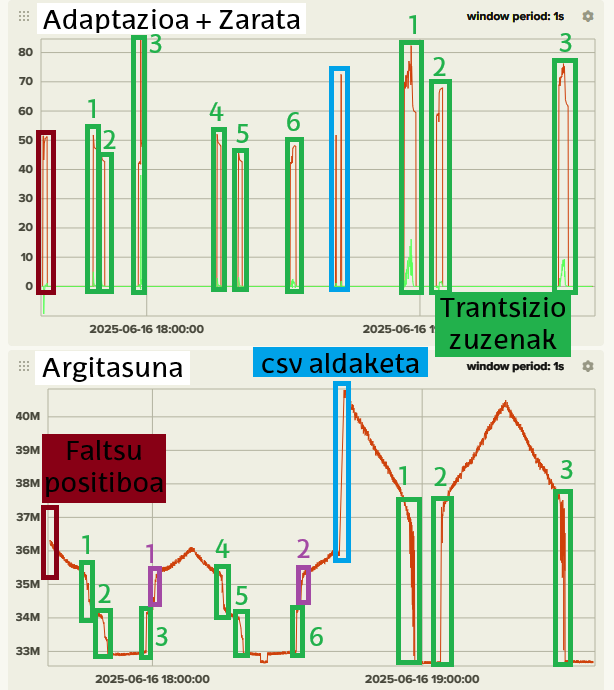
\includegraphics[width=0.8\linewidth]{5 - Zerbitzuaren garapena/influxdb_transitions.png}
    \caption{Adaptazioa eta zarata erabiliz detektatutako trantsizioak, argitasunarekin konparatuta \textit{InfluxDB}-n.}
    \label{fig:influxdb_transitions}
\end{figure}

\ref{fig:influxdb_transitions}. irudian ikus daitekeenez, adaptazioarekin antzemandako trantsizio gehienak argitasunean behatutakoekin bat datoz ($\%81.11$). Hala ere, bi ekorketa desberdinen arteko mugan ere trantsizioak detektatzen dira, nahiz eta benetakoak ez izan. Hori dela eta, garatutako zerbitzua datu errealekin testatzea ezinbestekoa da, sistemaren ekorketa desberdinekiko fidagarritasuna bermatzeko.\\

Horrez gain, \textit{Docker} edukiontziak etengabe zabaltzea praktikoa ez denez, trantsizio\hyp{}detekzioan parte hartzen duten funtzioen parametroak aukeratzeko eta doitzeko script gehigarri bat garatu da. Honek, datu historikoen \textit{.csv}-ak zeharkatzen ditu, datu-simulatzailearen antzera, eta zerbitzuaren fluxu berdina jarraituz, datu-leihoak puntu kopuruaren arabera definitzen dira. Trantsizio-detekzioa ahalik eta zehatzena izateko aukeratutako azkenengo balioak hurrengoak dira: \textbf{prom=0.5} eta \textbf{th=0.05}.\\

Horrela, atari balioak zehaztea askoz erosoagoa da, eta aukeraketa ez da estatikoa, beste edozein azeleragailura orokortu daiteke; nahikoa da \textit{.csv} berriekin elikatzea eta balioak probatzea trantsizioak ondo detektatzen diren arte.

\begin{figure}[h]
    \centering
    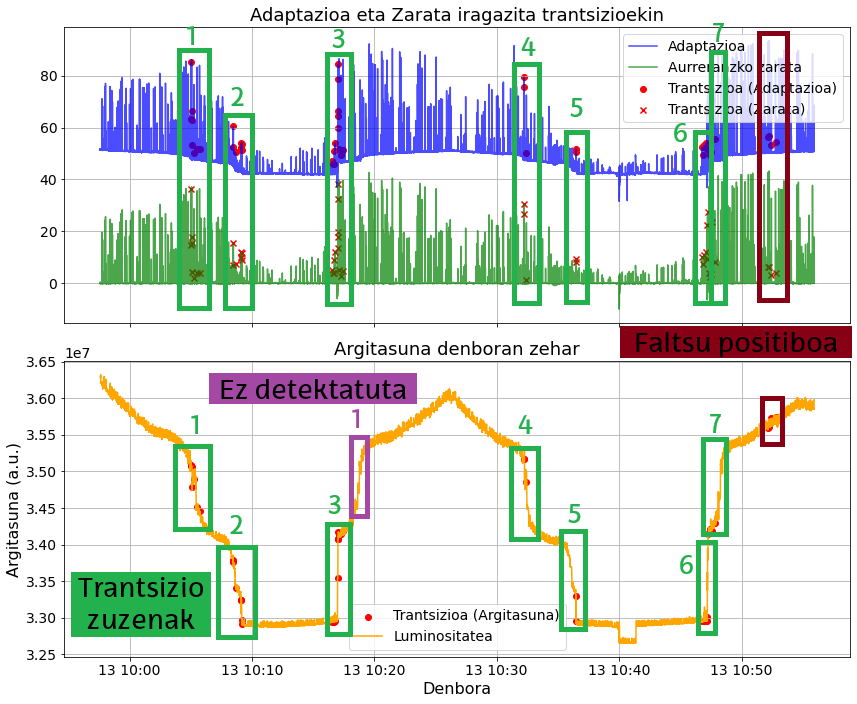
\includegraphics[width=0.85\linewidth]{5 - Zerbitzuaren garapena/offline_kalibrazioa.png}
    \caption{Offline kalibrazioaren adibidea, trantsizioak adaptazioaren bidez detektatuz.}
    \label{fig:offline_kalibrazioa}
\end{figure}

Dena dela, online zerbitzuan datuak denbora-tarteetan kontsultatzen direnez, eta offline script-an datu-kopuruaren araberako leihoak hartzen direnez, detektatutako trantsizio-kopuruak ez datoz guztiz bat: adibidez, lehenengo \textit{csv}-an (\ref{fig:offline_kalibrazioa}. irudia) eskuz 8 trantsizio bereiz daitezke, offline kalibrazioan 7 detektatzea lortzen da ($\% 87.5$), eta online zerbitzuan, berriz, 6 baino ez dira antzematen ($\%75$).

\subsection{Akatsen detekzioa}
Akatsak detektatzeko, trantsizioen programaren antzera, \textit{get\_data} funtzioaren bidez \textit{InfluxDB}-ko datuak kontsultatzen dira. Kasu honetan, ordea, akatsak edozein magnitudeetan antzeman daitezkeenez, magnitude guztiak jasotzen eta denboraren arabera ordenatzen dira.\\

Gainera, DBSCAN algoritmoan datuak dentsitatearen arabera multzokatzen direnez, denbora-leiho handiagoak hartuko dira, 800 segundokoak, datu kopurua handiagoa izateko, eta \textit{cluster}-ak dentsoagoak izateko. Datuen gainezarmena bermatzeko, berriz, \textbf{15 segundoero} deitzen da \textit{get\_data} funtzioa.

\begin{verbatim}
    from(bucket: "{bucket}")
            |> range(start: -800s)
            |> filter(fn: (r) => r["_measurement"] == "{measurement}")
            |> filter(fn: (r) => r["_field"] == "{field}")
            |> sort(columns: ["_time"])
\end{verbatim}

Bestalde, magnitudeak taldeetan banatu dira, ondoren DBSCAN talde horien gainean aplikatzeko. Banaketa honen bidez, fisikoki erlazionatuta dauden magnitudeak elkarrekin aztertzen dira, eta talde bakoitzarentzako \textit{eps} eta \textit{min\_samples} desberdin bat aukeratu daiteke, benetako anomaliak hobeto bereiziz.\\

Linac-7 azeleragailuaren kasuan, hiru talde bereizi dira, baina edozein azeleragailurako orokortu daitezke, soilik magnitudeen arteko lotura fisikoen arabera ezartzen baitira:

\begin{itemize}
    \item \textbf{RF-taldea}: Aurreranzko potentzia, Aurreranzko potentziaren erreferentzia eta Islapen-koefizientearen magnitudea.
    \item \textbf{Huts-taldea}: Gas-fluxua eta LEBT-eko presioa.
    \item \textbf{Argitasun-taldea}: Argitasuna isolatuta aztertu da.
\end{itemize}

Beraz, \textit{dbscan\_multi} funtzioa erabiliz, magnitude anitzeko taldeentzat DBSCAN aplikatzen da; argitasunaren talde isolatuarentzat, ordea, \textit{dbscan\_uni} funtzioa erabiltzen da. Algoritmoa aplikatu baino lehen, denbora-leiho bakoitzerako datuak \textit{scikit-learn} liburutegiko \textit{StandardScaler} tresna erabiliz normalizatzen dira: $\mu=0$ batezbestekoa eta $\sigma=1$ desbiderapen-estandarra ezartzen dira, algoritmoaren eraginkortasuna hobetzeko.\\

Orduan, lehen aipatutako \textit{eps} eta \textit{min\_samples} aldagaiak kontuan hartuz, \ref{sec:dbscan}. atalean aipatu den moduan, -1 etiketa duten puntuak lortzen dira, anomaliak. Azkenik, anomalien informazioa \textit{InfluxDB}-n argitaratzen da ere, \textit{anomalies} deituriko \textit{measurement} batean akatsa detektatu den taldearen magnitude guztiak gordez. Horrela, trantsizioen antzera, ikustarazpena errazten duten \textit{dashboard}-ak erraz sor daitezke.
\newpage
\begin{figure}[h]
    \centering
    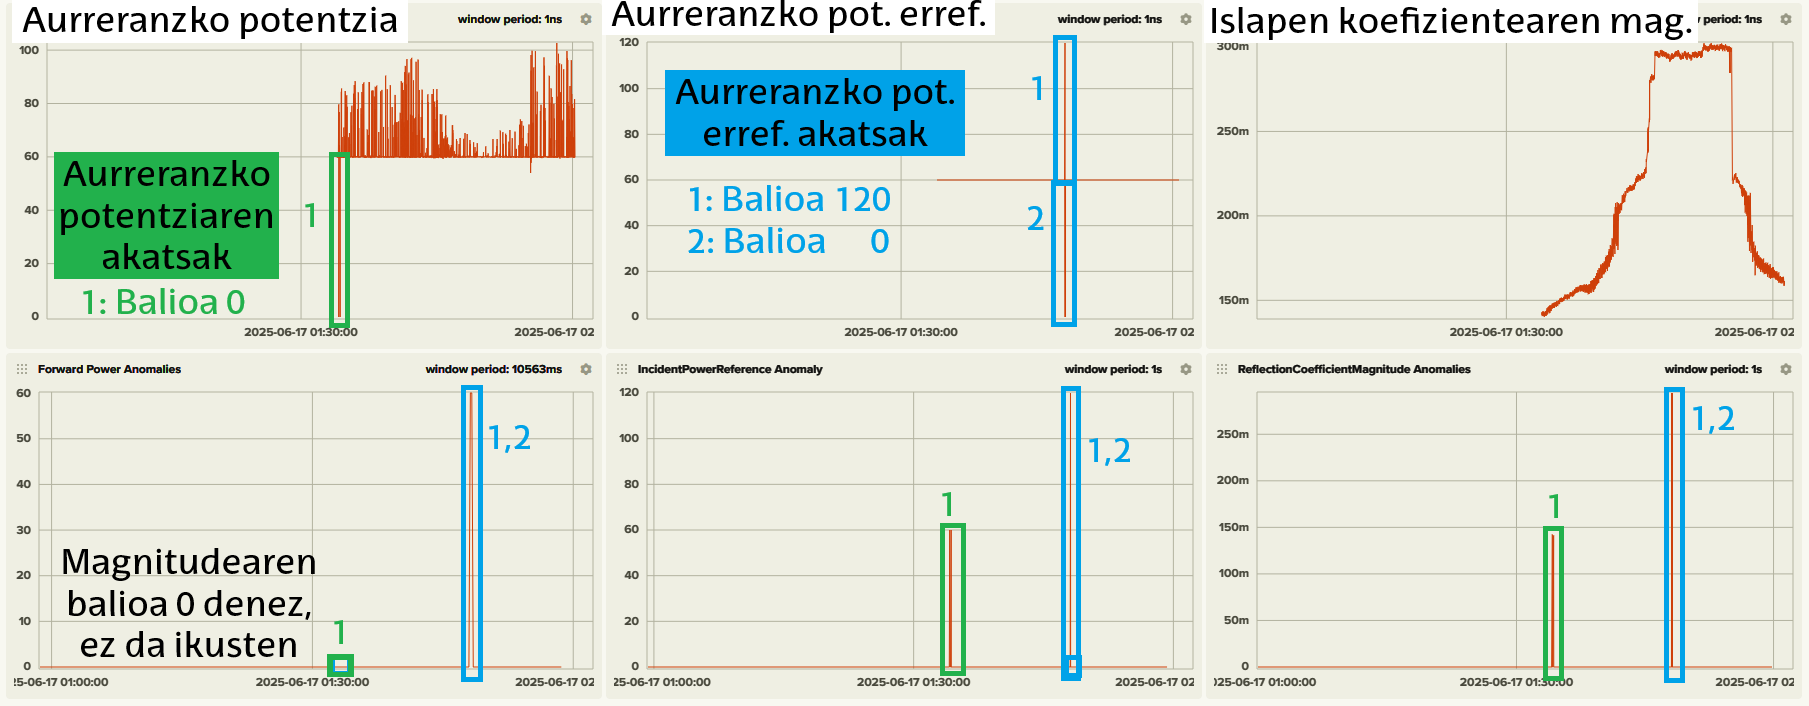
\includegraphics[width=\linewidth]{5 - Zerbitzuaren garapena/fault_dashboard_rf.png}
    \caption{DBSCAN erabiliz RF taldean detektatutako akatsak, \textit{InfluxDB}-n.}
    \label{fig:fault_rf}
\end{figure}
\begin{figure}[h]
    \centering
    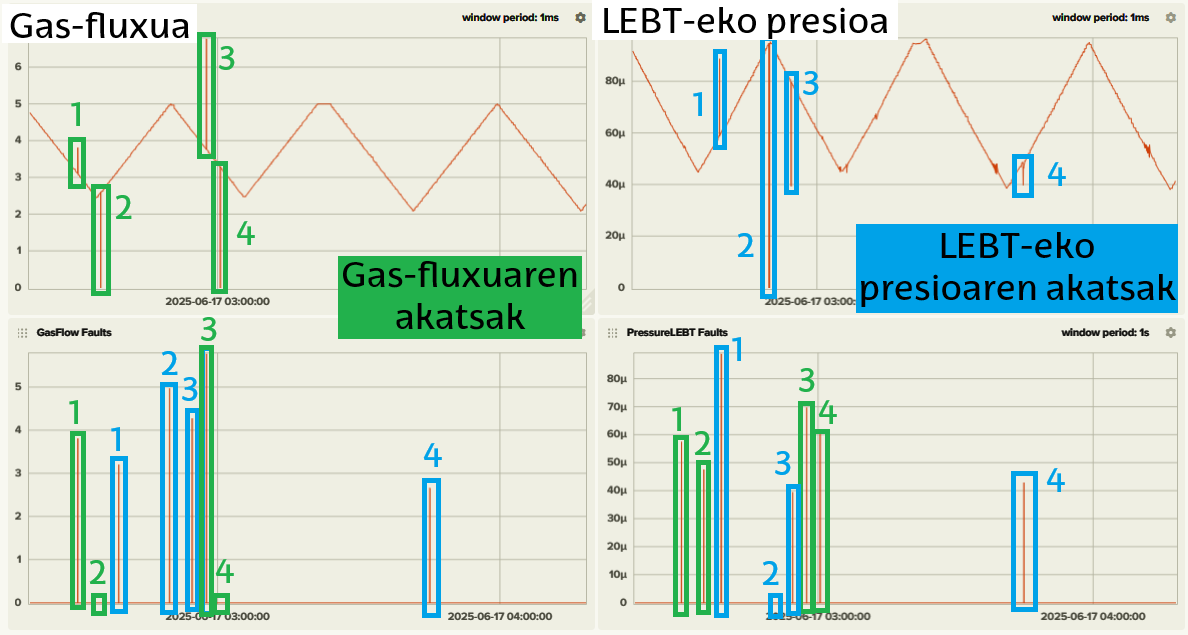
\includegraphics[width=\linewidth]{5 - Zerbitzuaren garapena/fault_dashboard_void.png}
    \caption{DBSCAN erabiliz huts taldean detektatutako akatsak, \textit{InfluxDB}-n.}
    \label{fig:fault_void}
\end{figure}

\ref{fig:fault_rf}. eta \ref{fig:fault_void}. irudietan ikus daitekeenez, RF eta huts taldeko akatsak zehaztasunez detektatzea lortzen da, eta baita informazioa gordetzea eta ikustaraztea ere. Hala ere, akatsen irudikapenerako magnitudeen balioa erabiltzen denez, hori 0 bada, puntua \textit{InfluxDB}-n gordetzen da, baina ez da baliorik ikusten. Ondorioz, anomaliak gordetzerakoan seinale digital berri bat definitzea eta gordetzea interesgarria da, akatsa antzematean 1 balioa hartzen duena, eta 0 beste edozein kasutan.\\

Bestalde, argitasunari dagokionez (\ref{fig:argitasuna_akatsak}. irudia), eskuz sartutako akatsak detektatu dira, baina horretarako aukeratutako \textit{eps} parametroa txikia izan denez, trantsizio zonaldeetan positibo faltsuak detektatzen dira; izan ere, bertan argitasunaren balioak aldaketa bortitzak jasaten dituenez, balioak ez daude behar bezain pilatuta, eta \textit{StandardScaler} bidez normalizatzerakoan sakabanatzen dira.
\newpage
\begin{figure}[h]
    \centering
    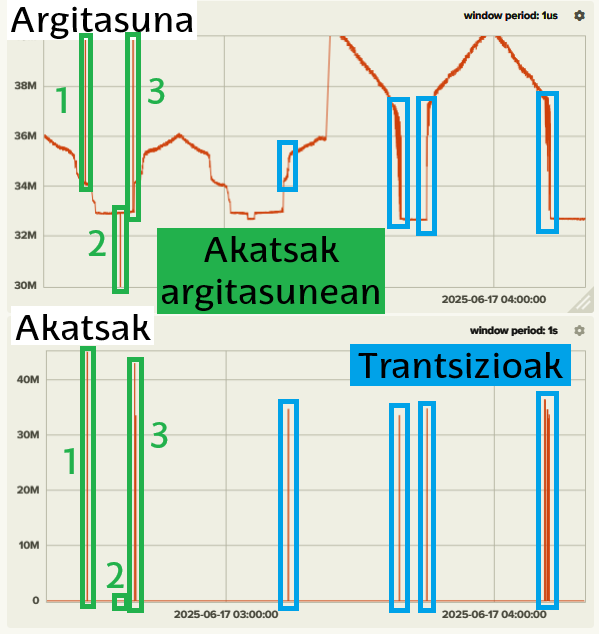
\includegraphics[width=0.6\linewidth]{5 - Zerbitzuaren garapena/fault_dashboard_argitasuna.png}
    \caption{DBSCAN erabiliz argitasunean detektatutako akatsak, \textit{InfluxDB}-n.}
    \label{fig:argitasuna_akatsak}
\end{figure}

Azkenik, funtzioen parametroak offline kalibratzeko script gehigarri bat garatu da kasu honetan ere. Trantsizioen detekziorako modu berean, datu historikoen \textit{.csv} fitxategiak zeharkatuz, DBSCAN datu-leihoetarako aplikatzen da, parametroen aukeraketa zuzeneko portamoldearekiko ahalik eta fidagarriena izateko. Akatsen detekzioa ahalik eta zehatzena izateko aukeratutako azkenengo balioak hurrengoak dira: \textbf{min\_samples=30}, $\mathbf{\epsilon_{RF}=14}$, $\mathbf{\epsilon_{V}=0.32}$ eta $\mathbf{\epsilon_{L}=0.6}$.\\

Gainera, programa honen bidez datuak bi dimentsiotan irudikatzeko aukera dago, datu-multzoen eta anomalien arteko banaketa argiago ikusteko (\ref{fig:dbscan_anomaliak_2}. irudia).
\begin{figure}[h]
    \centering
    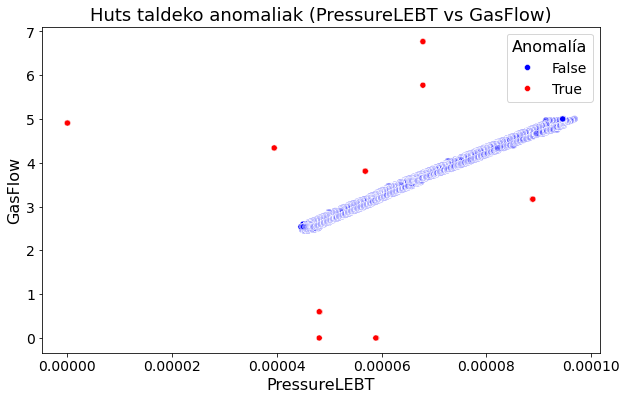
\includegraphics[width=0.6\linewidth]{5 - Zerbitzuaren garapena/dbscan_anomaliak2.png}
    \caption{Huts taldeko DBSCAN anomalia detekzioaren kalibrazioa offline.}
    \label{fig:dbscan_anomaliak_2}
\end{figure}
\newpage
\section{Ondorioak eta etorkizuna}
Lan honetan ECR ioi-iturrien plasma-trantsizioak eta sentsore akatsak modu ez-intrusiboan automatikoki detektatzeko zerbitzu bat garatu da, Linac-7 azeleragailuko azpiegituran eta datu-historikoetan oinarrituta. Horretarako, hauek izan dira landutako atalak, eta baita horietan lortutako ondorioak.\\

Lehenik eta behin, sistema garatzeko beharreko teknologiak aztertu dira: MQTT, Telegraf, InfluxDB eta Docker. Horiei esker, datuak modu azkar eta arinean jasotzeko, biltegiratzeko eta prozesatzeko azpiegitura orokor bat ezartzea lortu da, trinkoa eta modularra, edozein sistema eragiletara egokitzeko.\\

Ondoren, zerbitzuaren garapenerako erabilitako aldagaiak eta magnitudeak aurkeztu dira, Linac-7 proiektuko datu-historikoak erabiliz; izan ere, neurketa berriak zuzenean jasotzea ezinezkoa izan da ioi-iturriaren imanen akatsen ondorioz. Hala ere, horri aurre egiteko, datu-eskuratze simulatzailea garatu da, eta azeleragailuaren zuzeneko funtzionamendua imitatzea lortu da sare-lokalera konektatu gabe. Horrela, etorkizunean azeleragailuan arazo fisikoak izan arren, datu-prozesatzerako software berrien garapenak arazorik gabe jarraitu dezake.\\

Azkenik, trantsizio eta akats detekziorako aplikazioak garatu dira. Trantsizioei dagokienez, adaptazioa eta aurreranzko zarata zuzeneko diagnostiko ez\hyp{}intrusiborako erabilgarriak direla egiaztatu da, argitasunean behatutako trantsizio gehienak zehaztasunez hautemanez. Bestalde, akats detekziorako DBSCAN algoritmoa eraginkorra dela ondorioztatu da, datu-historikoetan eskuz sartutako anomaliak bereiztea lortu delako. Dena dela, bi detekzio-sistemen eraginkortasuna eskuz aukeratutako parametroen menpe dagoenez, ezinbestekoa da edozein azeleragailurako horiek offline kalibratzea.\\

Hori guztia kontuan hartuta, hasieran planteatutako helburuak bete dira, eta gainera, lanak hainbat erronka irekita uzten ditu, etorkizunean bai graduko bai graduondoko
ikerketetarako aukera emanez:

\begin{enumerate}
    \item Zerbitzua zuzeneko datuekin probatzea ezinbestekoa da. Gainera, PIT30 iturrirako iman berriak lortzen direnean, datu berriekin parametroen kalibrazioa egiaztatzea beharrezkoa da, azeleragailuaren ezaugarriak aldatu daitezkeelako.
    \item Zerbitzua beste azeleragailuetan testatzea interesgarria izango litzateke sistemaren orokortasuna berresteko. Zuzenean probatzea ezinezkoa bada, azeleragailu berrien datu-historikoak erabili daitezke probatzeko.
    \item Zerbitzuaren garapena gas-ekorketen datuekin egin denez, azeleragailuaren parametro operazionalak finkoak direnenean sistemaren funtzionamendua frogatzea funtsezkoa da ere.
    \item Trantsizio eta akatsen zuzeneko detekziorako beste teknika batzuk probatzea lagungarria izan daiteke, horien arteko zehaztasuna eta eraginkortasuna alderatzeko. Horrez gain, neurketa asko hartuz gero, Machine Learning teknikak garatzea posiblea da.
\end{enumerate}
\newpage
\section{Garapen Iraunkorrerako Helburuak}
Lan hau Nazio Batuen Erakundeko (NBE) Garapen Iraunkorrerako 2030 Agendako hainbat helburuekin lerrokatzen da:\\

\begin{itemize}
    \item \textbf{3. GIH: Osasuna eta ongizatea.} Linac-7 proiektuaren helburu nagusia PET (\textit{Positron Emission Tomography}) diagnostikorako erabiltzen diren isotopoak lokalki ekoiztea da. Gaur egun, aktibitate handiko eta erdibizitza luzeko isotopo garesti eta arriskutsuak erabiltzen dira, zentro espezializatuetan sortzen direnez ospitaleetaraino garraiatu behar baitira. Lan honen bidez, azeleragailu trinko eta merkeen garapena bultzatzen da, gaixoen tratamendu azkarragoa eta seguruagoa eskaintzeko.
    \item \textbf{4. GIH: Kalitatezko hezkuntza.} Lan honek ezagutza teknikoa euskaraz garatzea eta zabaltzea ere du helburu. Teknologia eta ingeniaritza bezalako arloetan euskararen presentzia mugatua denez, ezinbestekoa da maila altuko baliabide berriak euskaraz sortzea, hezkuntza-sistemaren kalitatea hobetzeko.
    \item \textbf{9. GIH: Industria, berrikuntza eta azpiegitura.} Lan honek berrikuntza teknologikoa sustatzen du sektore emergente batean: partikula-azeleragailuen diseinua eta automatizazioa. Azeleragailu trinkoen garapenak eta horietarako sortzen diren datu-prozesamendu eta diagnostiko automatikoen sistemak beste industrietarako eta ikerketarako aplikazio ugari dituzte, bai Euskal Herriko bai nazioarteko azpiegitura zientifiko eta teknologikoa sendotuz.
    
\end{itemize}

\newpage
\printbibliography

\end{document}
